\documentclass[a4paper]{book}
\usepackage{doc}
\usepackage{czech}
\usepackage{graphics}
\usepackage{amssymb}
\usepackage{makeidx}
\usepackage{times}
% \usepackage{doxygen/latex/doxygen}
\makeindex

\begin{document}

% hyperlink - mozna by stalo za to zdokonalit.

\def\href#1{{\it #1}}

\def\dia#1#2{
\begin{figure}[h]
\begin{center}
\scalebox{0.30}{\includegraphics{dia/#1.pdf}}
\end{center}
\caption{\label{fig:#1}#2}
\end{figure}}


\pagestyle{empty}


\begin{center}

	Univerzita Karlova v Praze

	Matematicko-fyzik�ln� fakulta


\vskip 0.5cm

\scalebox{.24}{
\includegraphics{mff.pdf}}

	Astronomick� �stav Akademie v�d �esk� republiky

	Ond�ejov

\vskip 0.5cm

\scalebox{.24}{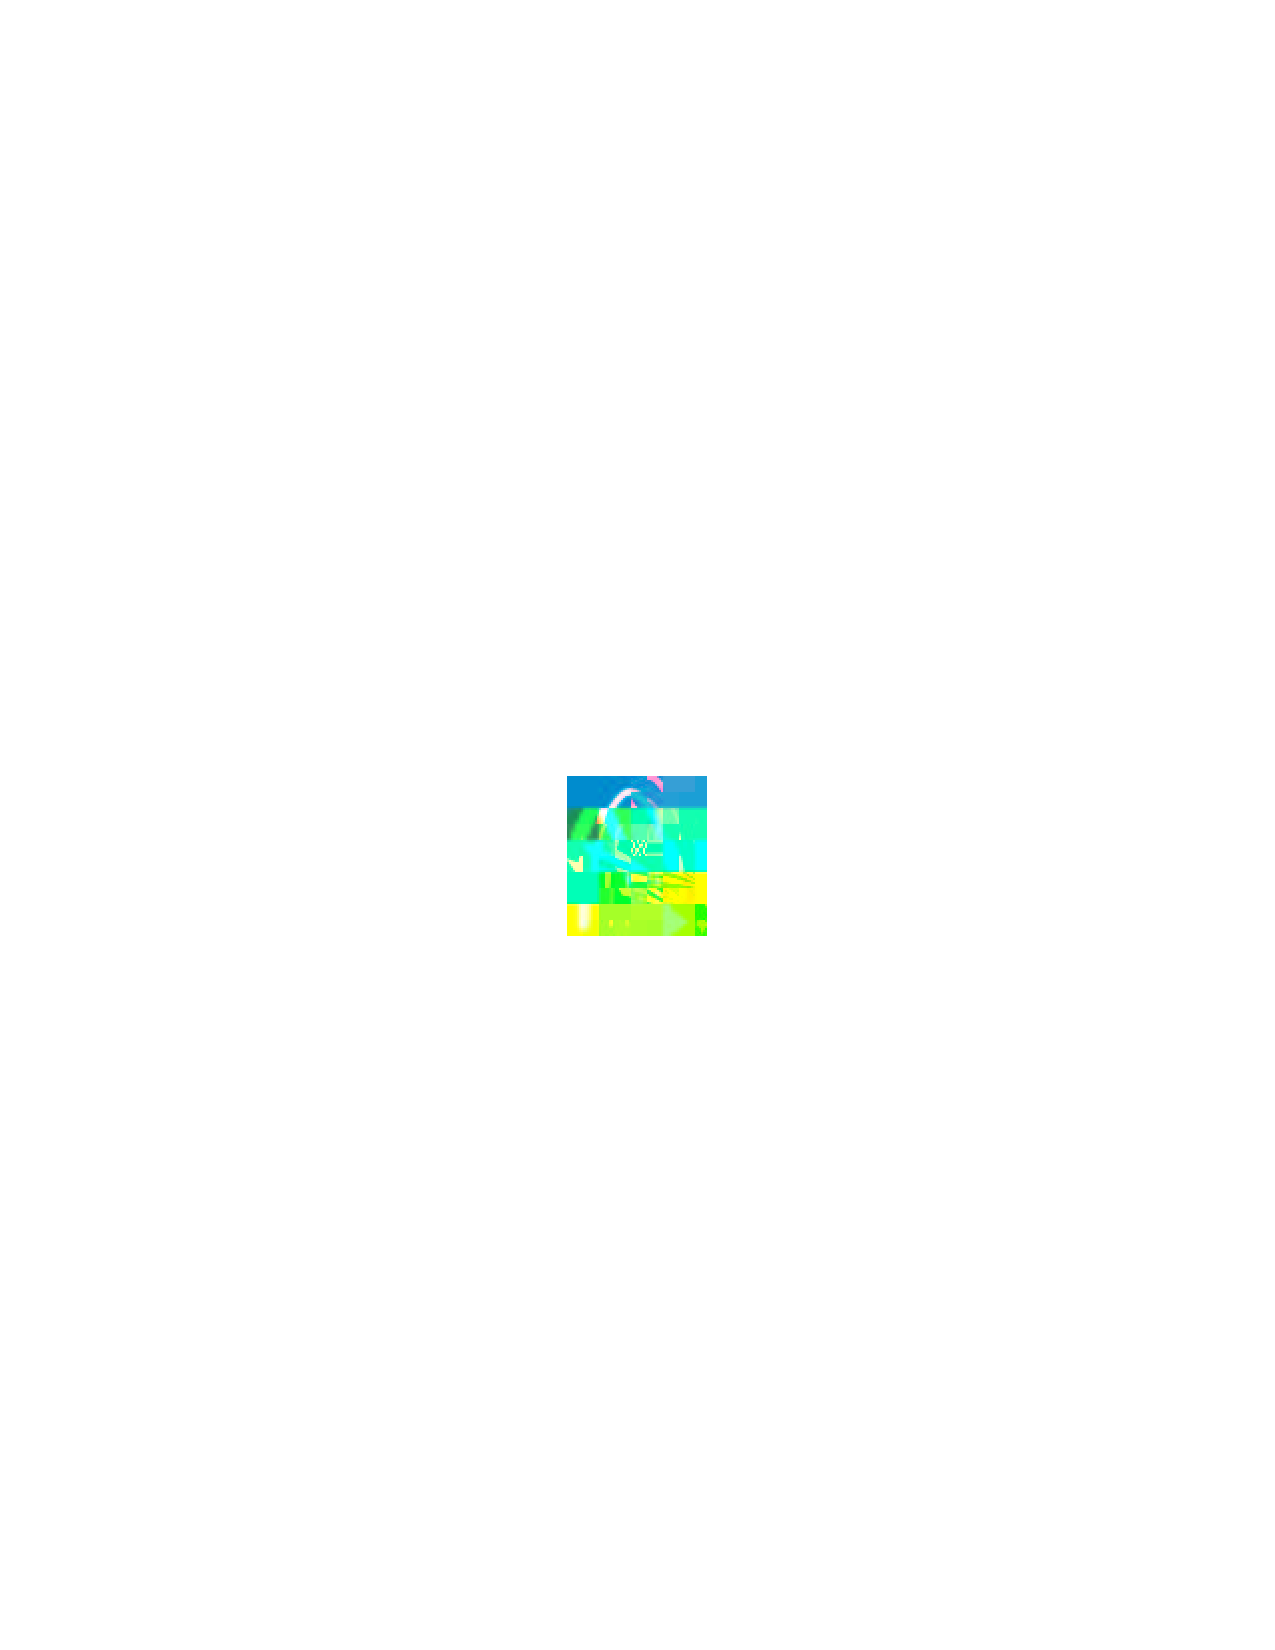
\includegraphics{asu.pdf}}

\vskip 1cm

	{\large \bf DIPLOMOV� PR�CE}

\vskip 2.5cm



	{\it Petr Kub�nek}

\vskip 0.3cm

	{\Large \it Zdokonalen� ��d�c�ho softwaru pro dalekohled BART}

\vfill

	{\it Katedra softwarov�ho in�en�rstv�}

	Vedouc� diplomov� pr�ce: {\it Mgr. Daniel ��oura�}

	Studijn� program: {\it informatika}

	{\it Softwarov� in�en�rstv�}

\vskip 2cm

\pagestyle{empty}

\end{center}


% �vod

{\it "Given that there are many telescopes, computers, and inventive
amateur and professional astronomers, it is only human nature that
successful attemps (and a few unsuccessful ones!) will be made to get
computer to control a telescope"} \\
\cite{telcontrol}
\newpage

\pagestyle{headings}
\pagenumbering{roman}
% obsah
\tableofcontents
% za��tek kapitol
\pagenumbering{arabic}
\noindent
{\bf Zad�n� diplomov� pr�ce}

\vspace{5mm}

\noindent Navrhn�te, implementujte a zdokumentujte ovl�d�n� dalekohledu BART (Burst
Afterglow Robotic Telescope) tak, aby umo��ovalo:

\begin{itemize}

\item ��zen� dalekohledu pomoc� p�edem spo��tan�ho pl�nu, s~mo�nost�
jeho p�eru�en� a p�ed�n� ��zen� jin�mu pozorov�n� v~p��pad� p��jmu
zpr�vy o~nov�m objektu, vhodn�ho k~okam�it�mu pozorov�n�

\item snadn� p�enos �e�en� na jin� kamery, p��padn� dalekohledy

\item on-line zpracov�n� sn�mk� na jin�m po��ta�i ne� na po��ta�i
obsluhuj�c�m kameru

\end{itemize}

Na z�v�r porovnejte nov� ovl�d�n� dalekohledu s~existuj�c�mi syst�my pro
ovl�d�n� dalekohled�.

% Je mo�n� vyu��t ovlada�e za��zen�, napsan� jako ��st ro�n�kov�ho projektu
% obh�jen�ho v~�ervnu 2000. Ostatn� k�d ro�n�kov�ho projektu nesm� b�t pou�it.
% Dokumentace k~pr�ci mus� obsahovat v��et k�du, p�evzat�ho z~ro�n�kov�ho
% projektu.
% 
% Pro �sp�n� vy�e�en� je t�eba prov�st n�sleduj�c� pr�ce
%
% \begin{itemize}
%
% \item definovat rozhran� pro ovl�d�n� za��zen� a p�enos dat z~nich,
%  prov�st jeho vzorovou implementaci na za��zen�ch, je� jsou
%k~dispozici na dalekohledu BART.
%
%\item vymyslet a naimplementovat pl�nova�, kter� bude ��dit pozorov�n�.
%
%\item zab�vat se ukl�d�n�m napozorovan�ch dat, jejich t��d�n�m a
%  zaji�t�n�m jednoduch�ho p��stupu k~nim.
%
%\item naimplementovat k~��stem, je� to vy�aduj�, grafick� u�ivatelsk�
%  rozhran�.
%
%\end{itemize}
%
%% \subsubsection{�asov� pl�n, sou�asn� stav}
%%
%%- definice rozhran�, vzorov� implementace - v~podstat� hotov�, dva
%%  t�dny �ist� pr�ce (stav�lo se na implementaci, kter� je k~dispozici
%%  pro dalekohled).
%%
%%- pl�nova� - ve f�zi �vah, jedna prototypov� implementace, trv�n� od m�s�ce
%%  do p�ti m�s�c�

%%- ukl�d�n� dat - ve f�zi �vah, z�le�itost do dvou t�dn� pr�ce
%%
%%- GUI - nen� zn�m kvantitativn� rozsah, t�ko se odhaduje, z�le�itost
%%  od t�dne po rok

\vspace{5mm}

{\it Konzultant}

\vspace{5mm}

Martin Jel�nek (mates@lascaux.asu.cas.cz), Astronomick� �stav Akademie v�d �esk� republiky, Ond�ejov 
% \\
% Renn� Hudec (rhudec@asu.cas.cz) \\
% Lenka �arounov� (lenka@asu.cas.cz) \\
% Jan Sold�n (soldan@asu.cas.cz)

\vspace{5mm}

{\it Literatura}
\nopagebreak
\vspace{5mm}
\nopagebreak

\noindent Martinez/Klotz - A~practical Guide to CCD astronomy \\
Trueblood/Genet - Telescope control, Willmann-Bell, 1997 \\
Mgr. R. Hal��, T. J�lek, P. Kub�nek, F. Krolluper, F. Kvapil - Detekce
astronomick�ch objekt� s~prom�nnou intenzitou za pomoci robotick�ho
teleskopu, Ro�n�kov� projekt MFF UK, Praha, 2000 \\
David Ratledge, The Art and Science of CCD Astronomy

\vspace{5mm}

{\it Odkazy}

\vspace{5mm}

\noindent {\bf http://www.telescope.org/rti/automated.html} p�ehled automatizovan�ch
dalekohled� \\
{\bf http://lascaux.asu.cas.cz} dalekohled BART \\
{\bf http://nova.sourceforge.net/} Projekt NOVA, automatick� ovl�d�n�
dalekohledu
{\bf http://www.astro.princeton.edu/\~{}bakos/HAT} The Hungarian Automated
Telescope

\vspace{5mm}

{\it Kvantitativn� po�adavky}

\nopagebreak
\vspace{5mm}

Po zad�n� a sezn�men� se s~probl�mem je vhodn� definovat m��iteln�
veli�iny, kter�ch by m�lo b�t dosa�eno.

- syst�m mus� reagovat na GRB zah�jen�m GRB pozorov�n� do 1 sekundy

- �as, kdy neb�� ��dn� pozorov�n�, nesm� p�es�hnout 10\% celkov�ho
pozorovac�ho �asu

\chapter{�vod}

\section{Pod�kov�n�}

Je t�k� ur�it, komu bych m�l pod�kovat v�ce a koho uv�st na prvn�m m�st�.
N�sleduj�c� seznam je neuspo��dan� a nemus� b�t nutn� �pln�. Pokud jsem v n�m
zapom�l n�koho uv�st, neu�inil jsem tak �mysln� a p�edem se mu za jeho
neuveden� omlouv�m.

Pod�kovat bych cht�l vedouc�mu diplomov� pr�ce, Danielovi ��oura�ovi.  Jednak
za jeho cenn� rady a p�ipom�nky, jednak za jeho trp�livost, kterou projevil
p�i neust�l�m odkl�d�n� term�nu zah�jen� �innosti na m� p�vodn� diplomov�
pr�ci, a n�sledn� p�i neust�l�m posouv�n� term�nu dokon�en� t�to diplomov�
pr�ce.

Za cenn� rady a p�ipom�nky pat�� d�k Martinovi Jel�nkovi. Bez diskuz� s n�m
bych nikdy nebyl schopen domyslet v�echny detaily. Neust�le m� upozornil na
vhodnost prov�d�t operace, kter� m� nenapadli ani v tom nejhor��m snu.

D�k za d�v�ru p�i psan� nov�ho k�du pat�� Renn�mu Hudcovi. Bez n�ho bych se
nav�c k dalekohledu BART v�bec nedostal a svoji diplomovou pr�ci bych asi
napsal na t�ma P�evody dynamick�ch UML model�, kter�to jsem m�l p�vodn�
zapsan�.

D�k za mater�ln�\footnote{ob�dy a ve�e�e p�i m�ch cest�ch na Ond�ejov},
jazykovou a v�emo�nou dal�� podporu pat�� m�m rodi��m.

V�em profesor�m Matematicko-fyzik�ln� fakulty pak pat�� m�j d�k za teoretick�
i praktick� znalosti, kter�mi m� b�hem m�ho pobytu na fakult� vybavili. Bez
teorie, jej�� v�znam jsem v po��tku nech�pal, bych nikdy nebyl schopen
pochopit a programovat ovl�d�n� dalekohledu.

Za moje hmotn� zaji�t�n� bych cht�l pod�kovat jedn� v�t�� zahrani�n� firm�.
D�ky jej�mu pom�rn� rozumn�mu p��stupu se m� snad poda�ilo zkombinovat studium
s prac�. Je z�ejm�, �e dan� spojen� negativn� ovlivnilo d�lku z�v�re�n� f�ze
m�ho studia, na druhou stranu m� vybavilo velk�m po�tem praktick�ch znalost�.

Za objevn� chyby a nedostatky v ovl�dan� mohou z velk� ��sti studenti
astronomie nebo zam�stanci AS�, kte�� s dalekohledem pozorovali. Pat�� mezi n�
Martin Topinka a Martin Nekola, jejich� vliv na �innost dalekohledu b�v�
katastrof�ln� a kte�� stoj� za v�t�inou odhalen�ch chyb. D�le mezi n� pat��
Jan Torman, Ond�ej Mikul��k, Iveta Stoklasov�, David Ond�ich, Marie Hrudkov�
a Libor Ba�ta.

D�k za skv�l� opera�n� syst�m a �irokou paletu n�stroj�, bez kter�ch bych
nebyl schopen ovl�d�n� dalekohledu kdy stvo�it, pat�� nezn�m�mu mno�stv�
program�tor� roztrou�en�ch po cel�m sv�t�.

Za programov�n� a spr�vu syst�mu pro distribuci informac� o zdroj�ch gama
z��en� pat�� d�k Steve Baco .. z Goddardova Space Flight Center.

Grantov� agentu�e AV �R a Evropsk� kosmick� agentu�e pak pat�� d�k za granty,
kter�mi je BART financov�n.

\section{Pou��v�n� astronomick�ch v�raz�}

Pro �sp�n� p�e�ten� a pochopen� t�to pr�ce je dobr� m�t z�kladn� znalosti
astronomick�ch v�raz� a v astronomii pou��van�ch pozi�n�ch syst�m�. Proto�e
jsou posp�ny v nespo�etn�m mno�stv� publikac� (nap��klad \cite{rts1} nebo l�pe
v \cite{telcontrol}, p�edpokl�d�m za zbyte�n� je opisovat.

\section{Gama z�blesky}

Gama z��en� je nejenergi�t�j�� elektromagnetick� z��en�. \index{Gama
Ray Burst}Gama Ray Burst, zkr�cen� \index{GRB}GRB, �esky \index{gama
z�blesky}gama z�blesky jsou prudk� a kr�tk� v�trysky tohoto z��en�,
p�ich�zej�c� k~n�m z~vesm�ru. Z�blesky trvaj� okolo jedn� sekundy.
Gama z��en� nepronikne zemskou atmosf�rou - gama z�blesky tedy mus�me
hledat pomoc� p��stroj� na dru�ic�ch.

Star�� dru�ice (COMPTEL, ..) poskytovali polohu zdroje Gama z�blesku pouze
p�ibli�n�, s chybou velikosti n�kolika stup��, nov� (HETE, INTEGRAL, Swift)
um� naj�t polohu zdroje Gama z�blesku pom�rn� p�esn� - chyba dosahuje
velikosti n�kolika minut.

\index{GRB!optick� prot�j�ek}Optick�m prot�j�kem gama z�blesku se
rozum� podez�el� objekt ve sm�ru gama z�blesku pozorovan� ve
viditeln�m spektru. Optick� prot�j�ek by podle teoretik� m�l b�t
pozorov�n u zhruba poloviny gama z�blesk�. M�l by b�t pozorovateln�
d�le ne� gama z�blesk - ur�it� minuty, mo�n� dny. Za jeden den mo�n� v pr�m�ru
detekovat je jeden gama z�blesk, z~r�zn�ch d�vod� (po�as�, um�st�n� na
neviditeln� ��sti oblohy, mal� jasnost, ..) u~v�t�iny nen� mo�no dohledat
jejich optick� prot�j�ky. Optick� dosvit zn�me u n�kolika des�tek GRB, co� je
mno�stv� neposta�uj�c� na vytvo�en� po��dn� statistky.

Nen� jasn�, z~�eho gama z�blesk poch�z� - existuje zhruba 200 teoretick�ch
model�. N�kter� z~nich p�edpokl�daj� katastrofick� sr�ky n�sledovan�
v�buchem. P�i sr�ce vznik� gama z��en�, p�i v�buchu z~n�raz�
rozp�naj�c�ch se ��stic poch�z� optick� z��en�. Optick� prot�j�ek by
m�l tedy b�t pozorovateln� o~trochu pozd�ji ne� gama z�blesk.
Z~extrapolace nam��en�ch optick�ch prot�j�k� gama z�blesk� vypl�v�, �e
by mohl m�t po kr�tkou dobu dostate�nou jasnost na to, aby byl
viditeln� i triedrem �i mal�m dalekohledem.

\section{Pozorov�n� GRB mal�mi dalekohledy}

Pro� m� smysl pozorovat oblasti, ve kter�ch byly detekov�ny gama
z�blesky, dalekohledy rozm�rov� podobn�mi tomu Ond�ejovsk�mu? D�vody
jsou n�sledujc�:

\begin{itemize}

\item velk� dalekohledy pozoruj� podle p�edem dan�ho pl�nu, nemaj� moc
volnosti pro p��padn� p�eru�en� pozorov�n�
\item mal� dalekohledy jsou levn�, lze jich tedy postavit v�ce a
pozorovat z v�ce m�st. Pozorov�n�m z v�ce m�st se zv���
pravd�podobnost �sp�n�ho pozorov�n�

\end{itemize}

Pro �sp�n� pozorov�n� je pot�eba splnit n�sleduj�c� podm�nky:

\begin{itemize}

\item na pozorovac�m stanovi�ti mus� b�t jasno a noc

\item pole, kter� se pozoruje, nesm� b�t v bl�zkosti m�s�ce; tato
podm�nka se st�v� kritickou pro pozorov�n� v �ase kolem �pl�ku.

\item dalekohled mus� b�t spr�vn� ustaven

\item cel� syst�m mus� reagovat spr�vn� a pozorov�n� prov�st

\end{itemize}

Ka�d� dalekohled nav�c, kter� je v provozu, tak m� sv�j v�znam. Umo��uje
rychlej�� detekci p��padn�ho optick�ho prot�j�ku, 

\section{Princip detekce gama z�blesk�}

Gama z��ezn� proch�z� pom�rn� snadno hmotou. Pokud se odraz� od
p�edm�tu, d�je se tak v n�hodn�m �hlu. Detektor tedy nelze stav�t
podobn� jako dalekohled.

Detektory pracuj� na dvou principech:

\begin{itemize}

\item pou��vaj� m���ku pro vytvo�en� obrazu

\item se znalosti �asu nesm�rov� detekce na dvou a v�ce bodech
dopo��t�vaj� poluhu zdroje

\end{itemize}

\ref{COMPTEL} a dru�ice \ref{IPN} byli vybaveny nesm�rov�mi detektory, nov�
dru�ice - \ref{HETE}, \ref{Integrla} a \ref{Swift} jsou vybaveny
m���kov�m detektorem.

\section{N�hradn� program}

Proto�e nelze o�ek�vat detekci gama z�blesku ka�dou noc, je vhodn� pro
dalekohled navrhnout n�hradn� program. Nejvhodn�j�� je monitoring
n�kolika vybran�ch zdroj�, s po��t�n�m jejich p�esn� fotometrie
\footnote{Fotometrie m��� jasnost hv�zd}.

Fotometrii lze d�lat bu�to relativn�, nebo absolutn�. Relativn�
spo��v� v porovn�v�n� jasnosti jedn� hv�zdy na n�kolika sn�mc�ch
po��zen�ch stejn�m p��strojem p�i pokud mo�no stejn�ch atmosf�rick�ch
prodm�nk�ch. Absolutn� fotometrie spo��v� v m��en� jasnosti v�ech
hv�zd na sn�m�, vypo�ten�m jejich p��strojov� magnitudy, ze znalosti
jasnosti kalibra�n�ch hv�zd dopo�ten�m jejich absolutn� magnitudy.

Absolutn� fotometrie je n�ro�n�j�� ne� relativn� fotometrie, jej�
p��nos je v�t��. Na BARTovi se sna��me o absolutn� fotometrii.

\section{RTS1}

Jako \index{RTS!RTS1}RTS1 je ozna�ov�n star� syst�m ��zen� dalekohledu,
vyvinut� v r�mci ro�n�kov�ho projektu student� MFF UK\ref{rts1}.
Zkratka \index{RTS} znamen� {\bf R}emote {\bf T}elescope {\bf S}ystem
\ref{rts1}.

\chapter{Design nov�ho ovl�d�n�}

\section{Co je na rts-1 �patn�}

\chapter{Design serveru}

\subsubsection{Stav}

Jsou k~dispozici atomick� funkce pro zm�nu stavu, a funkce pro jeho
p�e�ten�. Stav je um�st�n ve sd�len� pam�ti, tud�� je pro v�echny
instance serveru v�dy stejn�. Atomicita p��stupu k~n�mu je hl�d�na
pomoc� semafor�.

Informace o zm�n� stavu jsou ���eny pomoc� stavov�ch zpr�v v�em na za��zen�
p�ipojen�m klient�m.

\subsubsection{Spr�va vl�ken}

Pro vykon�v�n� funkc�, kter� trvaj� del�� dobu, se na serveru pou��vaj� 

\subsubsection{P�enos dat}

Data vznikaj� na po��ta�i, ke kter�mu je p�ipojena kamera. Odtud je
pot�eba je dostat n�kam na disk, do n�jak�ho prohl��e�e obr�zk�,
k~n�jak�mu zpracov�n�.

P�i vy��t�n� sn�mku je po��ta�, kter� vy��t�n� ��d�, zat��en natolik,
�e nem� moc v�znam uva�ovat nad n�jak� v�n�j��, na CPU n�ro�n�j��
anal�ze sn�mku.

Proto m� v�znam celou architekturu navhrnout tak, aby ke kame�e
(p��padn� kamer�m) byl p�ipojen po��ta�, kter� by slou�il jako server
- zpracov�val po�adavky na kameru a poskytoval odpov�di o~jej�m stavu.

\subsubsection{Jak ovl�dat za��zen�}

Na ovl�d�n� kamery budeme pot�ebovat minim�ln� jeden pln� duplexn�
komunika�n� kan�l. Vyu�ijeme n�jak�ho s��ov�ho protokolu, s~nejv�t��
pravd�podobnost� IP. 

Komunikovat m��eme bu�to pomoc� bin�rn� zak�dovan�ch zpr�v, nebo
rozhrann� zalo�en�m na telnetovsk�m (textov�m) protokolu - viz rfc854.

K�dovan� rozhrann� znamen� uzav�enost syst�mu, textov� rozhrann� je
mo�n� o~tro�ku slo�it�j�� implemetovat d�ky nutnosti dek�dovat p�ijat�
p��kazy, ale je otev�en�j��.

Rozhodl jsem se pro textov� rozhrann�. Jeho v�hody jsou otev�enost,
nez�vislost na architektu�e c�lov�ho po��ta�e\footnote{odpadaj� nap��klad
probl�my s konverz� dat mezi mal�mi a velk�mi endi�ny} a snadn� p�id�v�n�
dal��ch parametr� - v p��pad�, �e klient nebude rozum�t odpov�di serveru, m��e
j� prost� ignorovat. Pokud bych se rozhodl pro bin�rn� protokol, musel bych
zajistit schodnou verzi klient� a server�.

\subsection{P�enos dat}

Oby�ejn� stavov� data nen� probl�m p�ek�dovat do textov� podoby a poslat po
tomto rozhrann�, se sn�mky je to trochu hor�� - jsou to bin�rn� data ve
velikostech v ��du megabajt�, kter� by bylo z�hodno p�en�et rychle a
efektivn�.

Sn�mky, nebo sp��e obecn� bin�rn� data, je mo�n� p�en�et pomoc� n�kter�ho ze
standartn�ch protokol�. Data ulo��m do pam�ti, klientovi sd�l�m jejich
um�st�n� a klient si je od serveru pomoc� standartn�ho protokolu vy��d�.
Vhodn� protokoly by byli nap��klad FTP nebo HTTP, p��padn� zd�len� disk�
pomoc� NFS nebo Samby.

Druhou mo�nost� je n�vrh a implementace vlastn�ho protokolu.

P�enost dat pomoc� standartn�ch protokol� neumo��uje jejich streaming -
p�en�en� ��sti dat z kamery okam�it� po vy�ten� ��sti sn�mku. Tato vlasnost
se st�v� d�le�itou, pokud chceme po�izovat sn�mky v takzvan�m driftovac�m
re�imu, kdy je optika detek�n�ho p��stroje zam��ena na pevn� m�sto na obloze a
hodinov� posun mont�e je nahrazen vy��t�n�m ��dk� z kamery - po vy�etn�
jednoho ��dku se ��dky o jeden ��dek posunou, a na opa�n�m konci �ipu ne� z
kter�ho se vy��t� vznikne nov� ��dek.

P�enos dat p�es standartn� servery d�le vy�aduje existenci servru pro tento
protokol na za��zen�, ��d�c�m vy��t�n� kamery. Zv�t�uje tak po�adavky na pam�t
na stran� serveru. V p��pad�, �e by jsme se rozhodli �e�it vy��t�n�
jednoduch�m jedno��elov�m p��strojem, vy�aduje po n�s implemetaci tohoto
serveru i na dan� p��stroj.

P�i p�enosu dat p�es standartn� protokol je pot�eba zajistit jejich smaz�n�.
Vzhledem k tomu, �e klient m��e kdykoliv spadnou, p��padn� m��e doj�t k
p�eru�en� spojen�, nen� toto vhodn� �e�it vysl�n�m p��kazu ze strany klienta.

Rozhodl jsem se tedy pro vytvo�en� vlastn�ho protokolu pro p�enos dat, kter�
m� umo�n� streaming a nebude z�visl� na extern�m serveru.

Sn�mky, nebo sp��e obecn� bin�rn� data, je mo�n� p�en�et pomoc�
n�kter�ho ze standartn�ch protokol�. Data ulo��m do pam�ti,
klientovi sd�l�m jejich um�st�n� a klient si je od serveru pomoc�
standartn�ho protokolu vy��d�. Vhodn� protokoly by byli nap��klad FTP
nebo HTTP.

Sn�mky je ale vhodn� doplnit o 

Nab�zej� se dv� mo�nosti - sn�mky p�en�et po stejn�m spojen�, jako je
��d�c�, nebo pro p�enos sn�mk� vytv��et nov� spojen�. Mo�nost
vytv��et nov� spojen� se je�t� rozpad� na n�kolik variant podle toho, jak
podobn� spojen� navazovat, pou��vat, udr�ovat a ukon�ovat.

\subsubsection{Varianta jedno spojen�}

Na spojen� po�le server po po�adavku klienta data. Data budou zakon�ena
speci�ln� hodnotou, o kter� bude zn�mo, �e se jinde ne� na konci p�enosu
nevyskytuje. P��padn� server vy�le na za��tku spojen� informaci o velikosti
p�en�en�ch dat. T�m bude zaru�eno, �e klient pozn�, kdy data skon�ily, a
p�epne se zp�t do re�imu p�ij�maj�c�m odpov�di. Dal�� mo�nost� je vyhradit
��st dat pro stavov� informace - nap��klad do ka�d�ho n-t�ho bitu napsat
jedni�ku nebo 0 podle toho, jestli spojen� skon�ilo nebo ne. Na re�ii spojen�
pak padne 1/n-tina kapacity spojen�.

\begin{itemize}
\item{V�hody}
	\begin{itemize}
	\item jednoduch� na implementaci, jak na klientovi, tak na serveru
	\item nen�ro�n�
	\end{itemize}
\item{Nev�hody}
	\begin{itemize}
	\item na jednom spojen� nelze sou�asn� vy��tat data a pos�lat odpov�di na
	  stav za��zen�
	\item m�ch�n� textov�ch a binarn�ch dat m��e v�st ke zbyte�n�m probl�m�m
	  pro ��zen� p�enosu
	\end{itemize}
\end{itemize}

\subsubsection{Varianta ��d�c� a datov� spojen�}

Na ��d�c�m spojen� po�lu p��kaz, kter� ma data pos�lat. Jedna ze stran otev�e
datov� spojen�, druh� se k~n�mu p�ipoj�. Po nav�z�n� datov�ho spojen� ukon��m
�sp�n� vol�n� s~po�adavkem na data, od tohoto okam�iku mohu ��d�c� spojen�
znovu vyu��vat pro pos�l�n� dal��ch p��kaz�. Na datov� spojen� za�ne server
ps�t data, kter� klient vy��t�. Po posl�n� v�ech dat datov� spojen� ukon��m.

\begin{itemize}
\item{V�hody}
	\begin{itemize}
	\item mo�nost sou�asn� ovl�dat za��zen� a p�ij�mat data
	\end{itemize}
\item{Nev�hody}
	\begin{itemize}
	\item n�ro�n� na implementaci
	\end{itemize}
\end{itemize}

Rozhodl jsem se pro samostatn� datov� spojen�, rozhoduj�c�m faktorem byla
mo�nost pos�lat sou�asn� data a ovl�dat za��zen�.

P�i vlastn� implementaci jsem se inspiroval protokolem FTP, popsan�m v
\cite{RFC959}.

\subsection{Realizace}

Ka�d� server p�i startu �ek� na spojen� na TCP portu, na kter�m je
p�ipojen. Pokud takov� po�adavek p�ijde, forkne se, PID potomka
zaznamen� pro pozd�j�� pou�it�, a potomka zinicializuje. Potomek pak
mus� obslou�it v�echny do�l� po�adavky.

V�hod tohoto �e�en� je n�kolik:

\begin{itemize}
\item dostanu zadarmo nov�, zinicializovan� adresov� prostor
\item nemohu zasahovat do adresov�ho prostoru ostatn�ch spojen�
\item p��padn�mi chybami neovlivn�m ostatn� spojen�
\end{itemize}

P�i jeho realizaci je pot�eba zajistit komunikaci mezi centr�ln�m
serverem a procesy obsluhuj�c�my spojen�. Mo�nosti, kter� se nab�zej�:

\begin{itemize}
\item vytvo�it nov� spojen� na centr�ln� server
\item pou��t pro komunikaci s centr�ln�m serverem rodi�ovsk� proces, a
zajistit komunikaci s rodi�ovsk�m procesem
\end{itemize}

Prvn� mo�nost je dost nev�hodn� vzhledem k velk�mu mno�stv� dal��ch
spojen�, kter� bude pot�eba vytv��et a udr�ovat v chodu - ka�d�
spojen� na za��zen� znamen� jedno spojen� na za��zen�. Tedy,
konkr�tn�ji, pokud budu m�t k klient� a z za��zen�, budu vytv��et k*z
spojen�.

Druh� �e�en� je pouze odsunut� probl�mu o krok d�le. Ale sta�� m� v
n�m zajistit komunikaci mezi rodi�ovsk�m procesem a jeho potomky.  Co� nen�
zase tak velk� probl�m, na jeho vy�e�en� se nab�z� hned n�kolik metod:

\begin{itemize}
\item prost�edky IPC
\item obousm�rn� roury
\item unixov� sockety
\item TCP/IP sockety
\end{itemize}

TCP/IP sockety jsou uvedeny pouze pro �plnost. Vytv��en� a udr�ov�n� tohoto
typus pojen� vy�aduje nejv�ce syst�mov�ch prost�edk�, je v�hodn� pro
komunikaci p�es s��, ale je zbyte�n� pro komunikaci v r�mci jednoho po��ta�e.

Prost�edky IPC vypadaj� nejl�pe. Pomoc� rozli�en� p�es typ zpr�vy umo��uj�
doru�en� zpr�vy pouze vybran�mu p��jemci. Sd�len� pam�t m��e slou�it pro
ukl�d�n� informac�, ke kter�m pot�ebuj� p�istupovat jednotliv� spojen� -
nap��klad o stavu za��zen�. IPC semafory lze pou��t na hl�d�n� kritick� sekce
- z�pisu do sd�len� pam�ti.


\dia{state-serverd}{Stavov� diagram centr�ln�ho serveru}

\begin{description}

\item[on] ozna�en� pro mno�inu stav�, ve kter�ch je syst�m v norm�ln�m
provozu. Toto nen� stav

\item[off] stav, ve kter�m je cel� syst�m vypnut�. D�vodem pro vypnut� m��e
b�t nap��klad nep��zniv� po�as�, p��padn� technick� probl�my.

\item[day] den. Proto�e dalekohled je ur�en pro astronomick� pozorov�n�,
neb�� ��dn� �lohy. Lze pouze uva�ovat o prov�d�n� v�po�etn� n�ro�n�ch �kol�
souvisej�c�ch se zpracov�n�m dat z minul�ch pozorov�n�.

\item[evening] ve�er. Syst�m se p�ipravuje na pozorov�n�. P�echod do tohoto
stavu slou�� jako informace pro za��zen�, aby se p�ipravila k pozorov�n�.
Nap��klad se za�ne s chlazen�m kamer, otev�e se st�echa. Stav za��n� v pevn�
danou dobu p�ed z�padem Slunce.

\item[dusk] soumrak. Syst�m je p�ipraven na pozorov�n�. Obloha je sv�tl�, nem�
smysl prov�d�t dlouhodob� pozorov�n�. Lze prov�d�t pozorov�n� jasn�ch objekt�
- pokud dojde v tomto okam�iku ke gama z�blesku, m� v�znam ho pozorovat. Jinak
je vhodn� po�izovat kalibra�n� sn�mky.

\item[night] noc. Syst�m je pln� p�ipraven na pozorov�n�, obloha je temn�.
Pozoruje se. D�lka trv�n� stavu se schoduje s astronomickou noc�.

\item[dawn] rozb�esk. Stav podobn� soumraku, vhodn� pro pozorov�n� jasn�ch
objekt� nebo po�izov�n� kalibra�n�ch sn�mk�. Trv� od konce astronomick� noci
po v�chod Slunce.

\item[morning] r�no. Stav pro ukon�en� pozorov�n�. Vyp�n� se chlazen� kamer,
parkuje dalekohled, zav�r� st�echa, zpracov�vaj� korek�n� sn�mky.  Trv� od
v�chodu slunce po pevn� ur�enou dobu.

\end{description}


\subsection{Kamery}

\subsubsection{Stavov� diagram kamer}

\dia{state-camd}{Stavov� diagram CCD kamery}

\begin{description}

\item[noexposure] na dan�m �ipu neprob�h� ��dn� expozice

\item[exposing] prob�h� expozice

\item[data] na kame�e jsou k dispozici data, kter� je pot�eba vy��st

\item[reading] prob�h� vy��t�n� dat

\end{description}

\subsubsection{Chlazen� kamer}

V�echny nov�j�� astronomick� CCD kamery maj� zabudovan� chlazen�. Chlazen�
sni�uje teplotu CCD �ipu, a t�m sni�uje hodnotu temn�ho proudu. 

Temn� proud je tvo�en n�bojem, kter� se nashrom�d� na �ipu vlivem teplotn�ch
efekt� - tedy i v p��pad�, kdy� na �ip nedopad� sv�tlo. P�i po�izov�n� denn�ch
sn�mk� m��eme jeho efekt zanedbat - sn�mky maj� kr�tk� expozi�n� doby a vysok�
odstup sign�l/�um. Pro astronomick� sn�mky, kter� jsou po�izov�ny dlouhou
expozi�n� dobou a vyzna�uj� se mal�m odstupem sign�lu od �umu, je pot�eba
hodnotu temn�ho proudu co nejv�ce sn��it. �rove� temn�ho proudu z�vis� na
absolutn� teplot� �ipu, rozd�l mezi teplotou �ipu a teplotou okoln�ho
prost�ed� ji neovliv�uje.

Teplotn� regulace je v�t�inou tvo�ena pelti�rem a ventil�torem.  Pelti�r
p�en�� teplo z mal� plochy �ipu na ventil�tor, ventil�tor pak zlep�uje
distribuci tepla do okol�. Teplotn� regulace b�v� ob�as dopln�na o mo�nost
chlazen� vodou, p��padn� zkapaln�n�m plynem.

Expozici i vy�ten� sn�mku je vhodn� prov�d�t p�i konstantn� teplot� - nem�n�
se pak �rove� temn�ho proudu. Zm�ny teploty CCD �ipu trvaj� nenulov� �as,
teplota atmosf�ry se po z�padu Slunce v pr�b�hu noci zm�n� v�t�inou pouze o
n�kolik stup��. Po ka�d� zm�n� teploty je t�eba vy�kat, ne� se dostate�n�
prochlad� cel� CCD �ip.

Provoz RTS1 uk�zal, �e nem� smysl teplotu �ipu v pr�b�hu noci m�nit.  Syst�m
p�vodn� obsahoval k�d, kter� se sna�il optimalizovat c�lovou teplotu chlazen�
�ipu tak, aby se p��kon chlazen� dr�el v rozmez� doporu�ovan�ho v�robcem �ipu.
P�i zp�tn� kontrole sn�mk� po��zen�ch v pr�b�hu zm�ny teploty se uk�zalo, �e
sn�mky nemaj� line�rn� pr�b�h pozad� - prost�edek sn�mku m� hodnoty temn�ho
proudu vy��� ne� okraje pole. Tato nelinearita je zp�sobena rozd�lnou teplotou
okraje a st�edu CCD �ipu.

Aby bylo temn�ch sn�mk� pot�eba co nejm�n�, je vhodn� po�izovat sn�mky na co
nejmen��m po�tu teplot. U syst�mu BART se osv�d�ily p�tistup�ov� kroky.

\subsubsection{Nastaven� teploty kamery}

\dia{state-cooling}{Stavov� diagram chlazen� CCD kamery}

P�ed za��tkem pozorov�n� je spu�t�no chlazen� na maxim�ln� v�kon. V
okam�iku za��tku pozorov�n� je zji�t�na aktu�ln� teplota CCD �ipu
$ccd$, kter� je zaokrouhlena sm�rem nahoru k nejbli���mu stupni $step$ a na
tuto teplotu je nastaveno chlazen�. Obsluha m� mo�nost teplotu a v�kon chlazen�
kontrolovat, a podle pot�eby m�nit. Po skon�en� pozorov�n� nebo p�i vypnut�
syst�mu je chlazen� vypnuto.

Chlazen� m� tedy n�sleduj�c� stavy:

\begin{description}

\item[shutdown] chlazen� je vypnuto

\item[max] chlazen� b�� na maxim�ln� hodnotu, ventil�tor b��

\item[temp] chlazen� se sna�� udr�et teplotu �ipu na nastaven� hodnot�.

\end{description}

\subsubsection{Dostupn� informace}

\begin{itemize}

\item chlazen� kamery - c�lov� teplota, procentn� vyj�d�en� v�konu, teplota
�ipu, teplota okol�

\item velikost sn�man�ho pole

\item velikost v��ezu ze sn�man�ho pole

\end{itemize}


\section{teld}

\subsection{Stavov� diagram}

\begin{description}

\item[parked] mont� je zaparkov�na

\item[warp-drive] mont� se nepohybuje

\item[moving] mont� se pohybuje

\end{description}


\section{Dome}

\subsection{Stavov� diagram}

\begin{description}

\item[open] St�echa je otev�ena

\item[closed] St�echa je zav�ena

\item[opening] St�echa se otv�r�

\item[closing] St�echa se zav�r�

\item[good\_weather] po�as� umo��uje pozorov�n�

\item[bad\_weather] po�as� neumo��uje pozorov�n�

\end{description}


\section{Monitoring}

Monitoring poskytuje informace o stavu a hodnot�ch na jednotliv�ch
za��zen�ch.

D�le umo��uje volat v�echny funkce p�ipojen�ch za��zen�. Funkce lze
volat pomoc� notace:

\begin{center}
[ {jm�no za��zen�} . ]{p��kaz}
\end{center}

Jm�no za��zen� lze zjistit z panelu s informacemi o za��zen�. Ve�ker�
komunikace mezi nmonitoringem a p�ipojen�mi za��zen�mi se zobrazuje v
lev�m doln�m rohu.

Monitoring je napsan� s pou�it�m knihovny \cite{ncurses}.

\begin{figure}[ht]
\begin{center}
\scalebox{0.35}{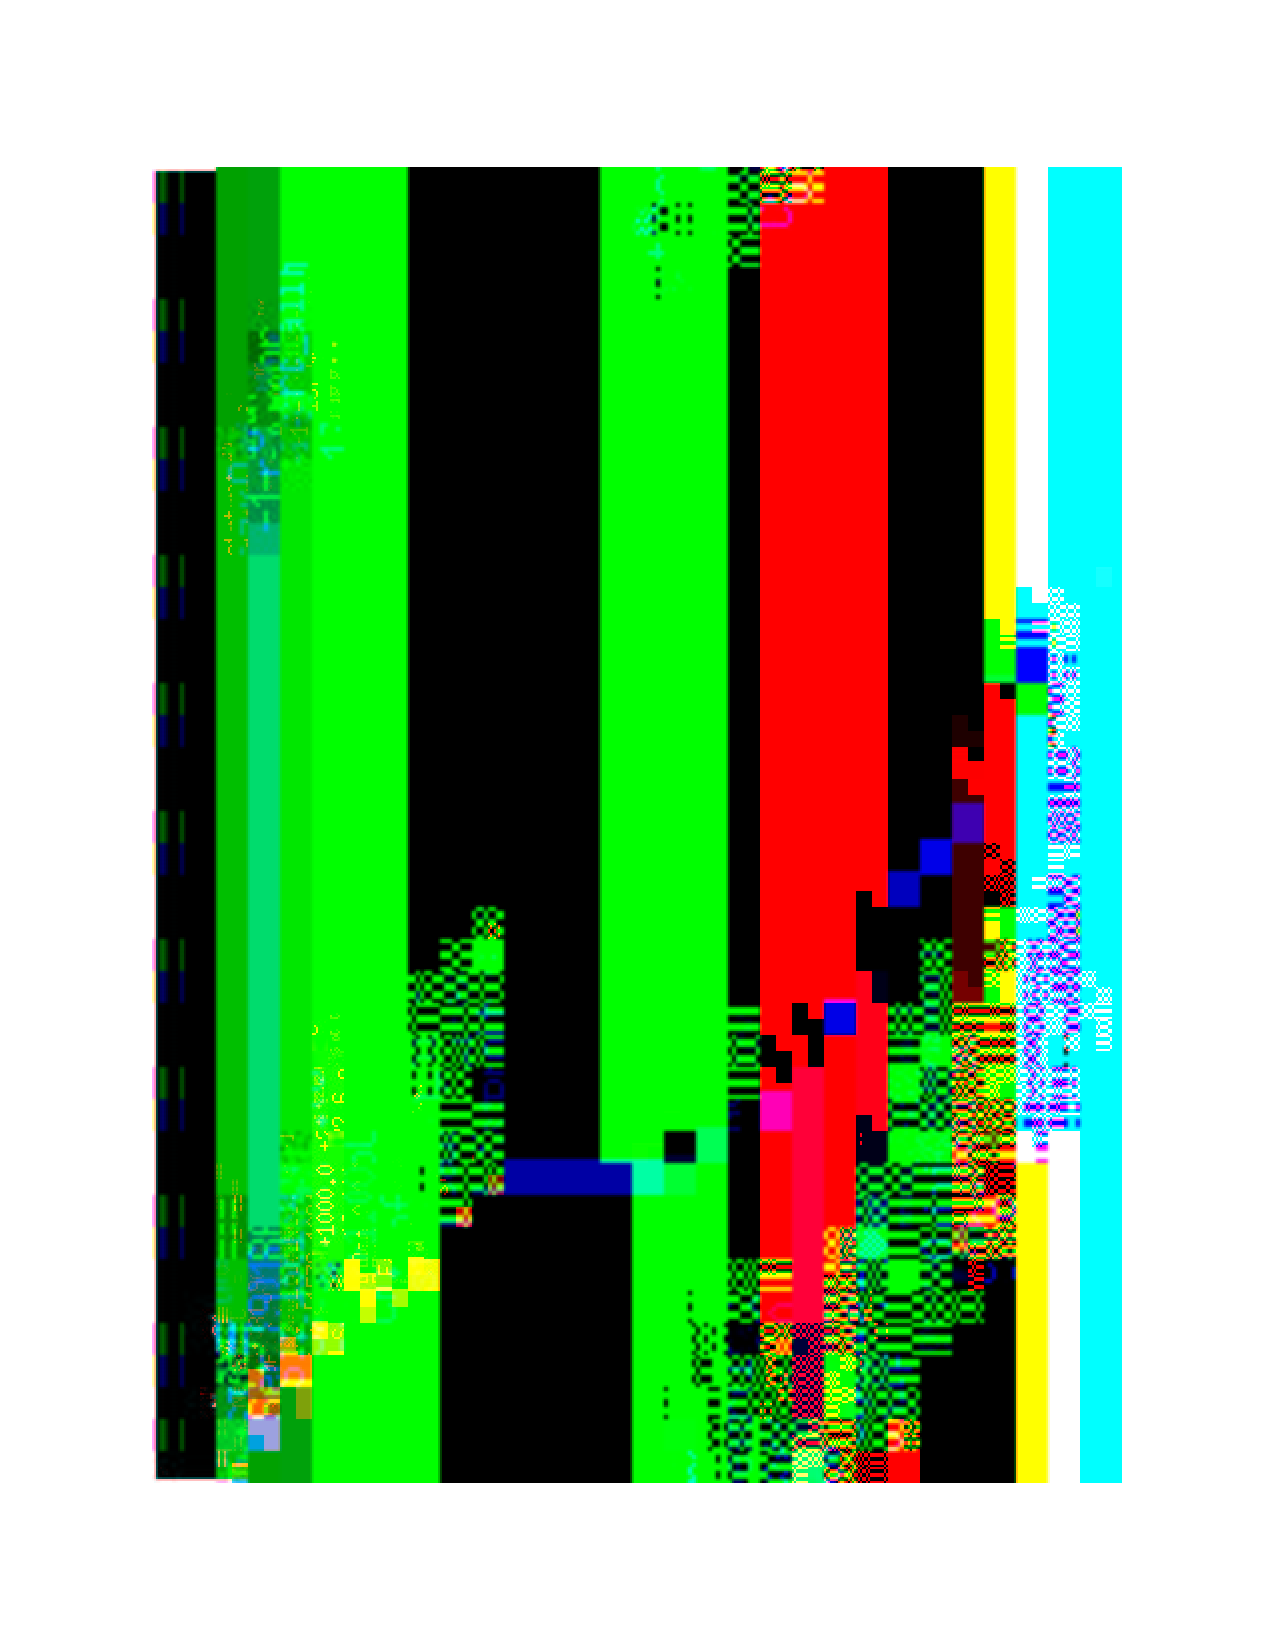
\includegraphics{nmonitor.pdf}}
\end{center}
\caption{\label{fig:nmonitor}Obrazovka nmonitoru}
\end{figure}


\section{Pl�nova�}

Pl�nova� ��d� dalekohled p�i dopl�kov�ch pozorov�n�. Pracuje s ni����
prioritou ne� klient pro p��jem zpr�v o z�blesku.

Pl�nova� vyb�r� c�le pozorov�n� z datab�ze, kter� obsahuje seznam
mo�n�ch pol�. Postup, pomoc� kter�ho se vyb�r� dal�� c�l pozorov�n�,
lze m�nit v soubru selector.ec.





\section{Distribuce zpr�v o pozorov�n� gama z�blesk�}

V�echny pozorov�n� gama z�blesk� jsou pos�l�ny na \ref{gcn}, odkud
jsou d�le distribuov�ny. GCN umo��uje pos�lat zpr�vy na email, pager
(zkr�cen� varianta emailu), nebo p�es vyhrazen� TCP/IP socket.

Pokud p�ij�m�me data p�es socket, doba jejich p��jmu z�vis� na stavu spojen� z
Ond�ejova na po��ta� GCN. V�t�inou se pohybuje do 1 sekundy.

P��jem dat p�es email trv� o trochu d�le, pr�m�rn� �as se pohybuje
kolem 30 vte�in. Zdr�en� je zp�sobeno zpracov�n�m emailu na po�tovn�ch
servrech.

Data p�ij�man� p�es socket nejsou opakov�na. Pokud spojen� nefunguje v dob�,
kdy dojde ke gama z�blesku, p�es socket se o n�j nedozv�me. Proto je vhodn�
zv�it mo�nost p��jmu dat p�es email jako z�lohu socketov�ho spojen� - email
doraz�, by� s �asov�m zpo�d�n�m, i p�i kr�tkodob�m v�padku sn�mku.

T�ko lze ��ci, jak dlouho po gama z�blesku m� smysl danou oblast pozorovat.
Lze uva�ovat o jednom dnu.



\chapter{Datab�ze}

P�esnou strukturu datab�ze - zvl�t� pak datov� typy jednotliv�ch polo�ek - je
mo�n� nal�zt v SQL skriptech, slou��c�ch pro vytvo�en� datab�ze, kter� jsou v
adres��i sql.

V n�sleduj�c�m textu jsou prim�rn� kl��e zna�eny zna�kou $\star$. Indexovan�
atributy jsou pak zna�eny pomoc� $\ast$.

\subsubsection{Tabulka epoch}

\begin{tabular}{ll}
{\bf $\star$ epoch\_id}	& identifikace epochy \\
{\bf epoch\_start}	& za��tek epochy \\
{\bf epoch\_end}	& konec epochy
\end{tabular}

\subsubsection{Tabulka targets}

\begin{tabular}{ll}
{\bf $\star$ tar\_id}	& ��slo c�le \\
{\bf type\_id}		& typ pozorov�n� \\
{\bf tar\_name}		& jm�no c�le \\
{\bf tar\_ra}		& rektascenze c�le \\
{\bf tar\_dec}		& deklinace c�le \\
{\bf tar\_comment}	& koment�� \\
\end{tabular}

\subsubsection{Tabulka types}

\begin{tabular}{ll}
{\bf $\star$ type\_id}	& ��slo typu \\
{\bf type\_description}	& popis
\end{tabular}

\subsubsection{Tabulka observations}

\begin{tabular}{ll}
{\bf $\ast$ tar\_id}	& ��slo c�le \\
{\bf $\star$ obs\_id}	& ��slo pozorov�n� \\
{\bf $\ast$ obs\_start}	& datum zah�jen� pozorov�n� \\
{\bf obs\_duration}	& d�lka trv�n� pozorov�n� \\
\end{tabular}

\subsubsection{Tabulka images}

\begin{tabular}{ll}
{\bf $\star$ img\_id}	& ��slo sn�mku \\
{\bf img\_name}		& jm�no sn�mku \\
{\bf $\ast$ img\_date}	& datum po��zen� sn�mku \\
{\bf img\_exposure}	& d�lka expozice \\
{\bf img\_temperature}	& teplota CCD �ipu \\
{\bf img\_filter}	& pou�it� filtr \\
{\bf astrometry}	& pozice sn�mku \\
{\bf $\ast$ obs\_id}	& ��slo pozorov�n� \\
{\bf camera\_name}	& jm�no kamery \\
{\bf mount\_name}	& jm�no mont�e \\
{\bf epoch\_id}		& ��slo epochy \\
{\bf media\_id}		& m�dium, na kter�m je sn�mek um�st�n
\end{tabular}

\subsubsection{Tabulka darks, flats}

\begin{tabular}{ll}
{\bf dark\_name}	& jm�no sn�mku \\
{\bf $\ast$ dark\_date}	& datum po��zen� sn�mku \\
{\bf dark\_exposure}	& d�lka expozice \\
{\bf dark\_temperature}	& teplota CCD �ipu \\
{\bf camera\_name}	& jm�no kamery
\end{tabular}

\vspace{1cm}

Tabulka flats obsahuje stejn� pole, pouze jejich prefix je flat.

\subsubsection{Tabulka cameras}

\begin{tabular}{ll}
{\bf $\star$ camera\_name}	& jm�no kamery \\
{\bf camera\_desc}		& popis kamery
\end{tabular}

\subsubsection{Tabulka mounts}

\begin{tabular}{ll}
{\bf $\star$ mount\_name}	& jm�no mont�e \\
{\bf mount\_long}		& zem�pisn� d�lka mont�e \\
{\bf mount\_lat}		& zem�pisn� ���ka mont�e \\
{\bf mount\_alt}		& nadmo�sk� v��ka mont�e \\
{\bf mount\_desc}		& popis mont�e
\end{tabular}

\subsubsection{Tabulka grb}

\begin{tabular}{ll}
{\bf tar\_id}		& ��slo pozorov�n� \\
{\bf $\star$ grb\_id}	& ��slo GRB \\
{\bf grb\_seqn}		& aktu�ln� ��slo po�ad� zpr�vy \\
{\bf grb\_date}		& datum pozorov�n� GRB \\
{\bf grb\_last\_update}	& datum posledn� zm�ny stavu GRB \\
\end{tabular}

\subsubsection{Tabulka ot}

\begin{tabular}{ll}
{\bf tar\_id}		& ��slo pozorov�n� \\
{\bf ot\_imgcount}	& po�et sn�mk� po�adovan�ch za jednu noc \\
{\bf ot\_minpause}	& minim�ln� rozestup mezi sn�mky \\
{\bf ot\_priority}	& priorita pozorov�n� \\
\end{tabular}

\subsubsection{Tabulka medias}

\begin{tabular}{ll}
{\bf $\star$med\_id}	& identifika�n� ��slo m�dia \\
{\bf med\_path}		& cesta, na kter� je m�dium namontov�no \\
{\bf med\_mounted}	& logick� hodnota, ur�uj�c�, jestli je dan� m�dium namontov�no
\end{tabular}

\vspace{1cm}

V datab�zi je definov�n u�ivatelsk� typ, kter� slou�� pro ukl�d�n� informace o
poloze sn�mku. Je odvozen ze struktury, pou��van� v knihovn� libwcs. Obsahuje
informace o poloze referen�n�ho bodu sn�mku, jeho sou�adnic�ch, rozm�rech
pixelu, rotaci sn�mku a parametry korek�n�ho polynomu, kter� slou�� pro
v�po�et sou�adnic ostatn�ch bod� na sn�mku.

V datab�zi jsou d�le implementov�ny funkce, slou��c� jednak k obsluze
u�ivatelsk�ho typu pro ukl�d�n� sou�adnic sn�mku, a jednak k transformac�m
ekliptik�ln�ch sou�adnic na horizont�ln�, a v�po�et vzdu�n� hmoty.

\chapter{Implementace}

\section{C�lov� platforma}

C�lovou platformou jsou po��ta�e zalo�en� na procesorech i386.

Pou��van�m opera�n�m syst�mem je GNU Linux. Pou��vali jsem distribuce RedHat,
Mandrake a Debian. D�ky propracovan�mu bal�kovac�mu syst�mu se jako nejlep��
jev� Debian. Ten v sou�asn� dob� nasazujeme na v�echny nov� po��ta�e.

Komunikace mezi po��ta�i b�� na s��ov�m protokolu TCP/IP. D�vodem je jeho
roz���enost.

\section{C�lov� jazyk}

V�t�ina k�du je naps�na v jazyce C, tedy bez pou�it� objekt�. Datab�zov�
operace jsou pops�ny v jazyce SQL. Webovsk� str�nky jsou psan� v jazyce PHP. Integra�n� ��sti k�du jsou ps�ny v bash skriptech.

\section{Protokol}

V n�sleduj�c�m textu je za {\bf server} ozna�ov�n proces, kter� �ek� na
spojen�. Jako {\bf klient} je pak ozna�ov�n proces, kter� spojen� otv�r�.

Je pot�eba rozli�ovat klienty pro jednotliv� �innosti (monitoring, ..) s
klienty v protokolu.  

Proces centr�ln�ho serveru vystupuje v protokolu pouze jako sever. 

Klientsk� procesy vystupuj� v protokolu v�dy jako klienti.  

Za��zen� vystupuj� p�i komunikaci se za��zen�my jako server. P�i komunikaci s
centr�ln�m server pak vystupuj� jako klient. A p�i komunikaci mezi za��zen�my
se jedno chov� jako klient a druh� jako server.

\subsection{Form�t}

Komunikovat m��eme bu�to pomoc� bin�rn� zak�dovan�ch zpr�v, nebo rozhrann�
zalo�en�m na textov�ch zpr�v�ch.

Bin�rn� komunikace je t�k� pro pochopen� p�i pohledu zven��, vy�aduje
pou��v�n� p�esn�ch vol�n�. Bin�rn� komunikace je sv�z�na s architekturou, na
kter� funguje. P�i jej�m p��jmu na jin� architektu�e je zapot�eb� j� nejd��ve
konvertovat.

Textov� rozhrann� lze p�i pohledu zven�� snadno pochopit. Je n�ro�n�j�� na
syst�mov� prost�edky ne� bin�rn� komunikace - p�en�ej� se del�� data, p�ijat�
p��kazy je pot�eba p�ed zpracov�n�m detekovat.

Syst�m pou��v� pro p�enos p��kaz� a zpr�v textov� komunikace. Pro p�enos
bin�rn�ch dat (sn�mk�) se pou��v� bin�rn�ho form�tu.

Bloky komunikace v textov�m rozhrann� jsou ukon�ov�ny zna�kou konce ��dky.
Bu�to se pou��v� znak� platn�ch v protokolu Telnet \cite{telnet} - tedy znaku
CR n�sledovan�ho znakem LF, nebo pouze znaku LF.

Jednotliv� polo�ky ��dky jsou odd�lov�ny nejm�n� jedn�m znakem mezera.

\subsection{P��kazy}

P��kazy pos�l� klient serveru. Prvn� polo�kou ��dku je n�zev p��kazu.
N�zev p��kazu je n�sledovan parametry.

Na jedn� ��dce je mo�n� poslat n�kolik p��kaz�. Jako jejich odd�lova� slou��
st�edn�k.

\subsection{Odpov�di}

Server na p��kazy odpov�d�. Odpov�� serveru je v�dy zakon�ena ��dkou,
za��naj�c� znakem '+' nebo '-' a pokra�uj�c� stavov�m k�dem slo�en�m ze t��
��slic. Server za�ne dal�� p��kaz p�ijat� od klienta zpracov�vat a� po
odesl�n� zakon�ovac� ��dky.

Pokud je prvn�m znakem zakon�ovac� ��dky '+', p��kaz byl �sp�n� vykon�n.
Pokud je t�mto znakem '-', p��kaz skon�il chybou. Podle stavov�ho k�du lze pak
rozli�it, o jakou chybu se jednalo.

��dky obsahuj�c� hodnotu za��naj� mal�m p�smenem. Pos�l� je server klientovi,
v�t�inou jako reakci na p��kaz a tedy p�ed t�m, ne� ozn�m� ukon�en� p��kazu.
Prvn� polo�ka je jm�no p��kazu, za n� n�sleduj� hodnotami. 

Nap��klad po dotazu na pozici dalekohledu m��e dalekohled odpov�d�t{\it ra
10}, co� znamen�, �e je v rektascenzi nastaven na 10 stup��.

\subsection{Zpr�vy a ��dosti serveru}

��dky, kter� pos�l� server klientovy a kter� za��naj� velk�m p�smenem obsahuj�
bu�to zpr�vy, nebo ��dosti serveru. Mohou se vyskytovat kdykoliv v pr�b�hu
komunikace klienta se serverem. Klient jejich p��jem nepotvrzuje.

\subsubsection{Stavov� zpr�vy}

Za��naj� znakem 'S', a obsahuj� n�zev stavu, jeho novou hodnotu a dopl�uj�c�
koment��.

\subsubsection{Otev�en� datov�ho spojen�}

��dosti na otev�en� nov�ho datov�ho spojen� za��naj� znakem 'D'. Pot�
n�sleduje �et�zec connect, jm�no nebo IP adresa a port, na kterou se m� klient
p�ipojit. Posledn� je d�lka bloku p�en�en�ch dat.

Klient by se po p�ijet� t�to ��dosti m�l pokusit o nav�z�n� spojen� na danou
s��ovou adresu.

\subsubsection{Zpr�vy}

Zpr�vy za��naj� p�smenem M, za kter�m n�sleduje text zpr�vy.

\subsubsection{Informa�n� zpr�vy}

Za��naj� p�smenem I. Informuj� klineta o zm�n� po�tu a hodnot�ch stavu
serveru, a o p�ipojen�ch klientech.


\section{Komunika�n� knihovna}

Komunika�n� knihovna mus� spl�ovat n�sleduj�c� po�adavky:

\begin{itemize}
\item umo��ovat pos�l�n� zpr�v
\item umo��ovat p�enos velk�ch objem� bin�rn�ch dat
\item podporovat model klient - centr�ln� server - za��zen�
\item kl�st mal� n�roky na syst�mov� prost�edky
\end{itemize}

Syst�m pou��v� vlastn� komunika�n� knihovny.

\subsection{Architektura komunika�n� knihovny}

Knihovna se skl�d� z n�sleduj�c�ch ��st�:

\begin{description}
\item[devser] knihovna pro server
\item[devcli] knihovna pro klienty
\item[devdem] knihovna pro za��zen�
\end{description}

\subsection{devser}

Slou�� pro serverovou stranu spojen�. Poskytuje funkce nutn� pro p�e�ten�
p��kazu a zpracov�n� p��kazu, posl�n� odpov�di a zakon�ovac� ��dky p��kazu.

\subsection{devcli}

Slou�� pro klientskou stranu spojen�. Poskytuje funkce pro nav�z�n� komunikace
se serverem, posl�n� p��kazu na servera, zpracov�n� a p�e�ten� odpov�d� ze
serveru. Zpracov�v� v�echny po�adavky a zpr�vy serveru, pokytuje p��stupov�
body pro funkce pro p��jem dat a funkce volan� p�i zm�n� stavu.

Udr�uje komunikaci s centr�ln�m servrem, zji��uje stavy a po�et za��zen�.

\subsection{devdem}

Integruje devcli a devdem. Poskytuje podporu pro za��zen�.

\subsection{Architektura serveru}

Pro ka�d� nov� spojen� je vytv��en a spou�t�n nov� proces. Pro synchronizaci
server� a jejich vz�jemnou komunikaci jsou pou�ity prost�edky IPC.

Pro d�letrvaj�c� operace je vytv��eno nov� vl�kno. Vl�kna jsou vytv��ena
pomoc� knihovny pthread.

\section{Zpracov�n� sn�mku}

Pro zpracov�n� sn�mk� je vol�n shellovsk� skript. Pokud se na jeho v�stupu
vyskytne ��dka s �daji o skute�n� pozici sn�mku a velikosti chyby, je chyba
posl�na na dalekohled.

Sn�mky se po po��zen� �ad� do z�sobn�k�, z kter�ho je odeb�r�n k�dem pro
zpracov�n� sn�mk�. Je garantov�no, �e v jednom klientu pob�� pouze jeden
proces pro zpracov�n� sn�mk�.

O detekci hv�zd se v syst�mu BART star� program sextractor. Jeho konfiguraci
provedl Martin Jel�nek.

O srovn�n� detekovan�ch hv�zd s katalogem se star� bal�k Opera, vyvinut� ....
a upraven� Martinem Jel�nkem.


\chapter{Design serveru}

\subsubsection{Stav}

Jsou k~dispozici atomick� funkce pro zm�nu stavu, a funkce pro jeho
p�e�ten�. Stav je um�st�n ve sd�len� pam�ti, tud�� je pro v�echny
instance serveru v�dy stejn�. Atomicita p��stupu k~n�mu je hl�d�na
pomoc� semafor�.

Informace o zm�n� stavu jsou ���eny pomoc� stavov�ch zpr�v v�em na za��zen�
p�ipojen�m klient�m.

\subsubsection{Spr�va vl�ken}

Pro vykon�v�n� funkc�, kter� trvaj� del�� dobu, se na serveru pou��vaj� 

\subsubsection{P�enos dat}

Data vznikaj� na po��ta�i, ke kter�mu je p�ipojena kamera. Odtud je
pot�eba je dostat n�kam na disk, do n�jak�ho prohl��e�e obr�zk�,
k~n�jak�mu zpracov�n�.

P�i vy��t�n� sn�mku je po��ta�, kter� vy��t�n� ��d�, zat��en natolik,
�e nem� moc v�znam uva�ovat nad n�jak� v�n�j��, na CPU n�ro�n�j��
anal�ze sn�mku.

Proto m� v�znam celou architekturu navhrnout tak, aby ke kame�e
(p��padn� kamer�m) byl p�ipojen po��ta�, kter� by slou�il jako server
- zpracov�val po�adavky na kameru a poskytoval odpov�di o~jej�m stavu.

\subsubsection{Jak ovl�dat za��zen�}

Na ovl�d�n� kamery budeme pot�ebovat minim�ln� jeden pln� duplexn�
komunika�n� kan�l. Vyu�ijeme n�jak�ho s��ov�ho protokolu, s~nejv�t��
pravd�podobnost� IP. 

Komunikovat m��eme bu�to pomoc� bin�rn� zak�dovan�ch zpr�v, nebo
rozhrann� zalo�en�m na telnetovsk�m (textov�m) protokolu - viz rfc854.

K�dovan� rozhrann� znamen� uzav�enost syst�mu, textov� rozhrann� je
mo�n� o~tro�ku slo�it�j�� implemetovat d�ky nutnosti dek�dovat p�ijat�
p��kazy, ale je otev�en�j��.

Rozhodl jsem se pro textov� rozhrann�. Jeho v�hody jsou otev�enost,
nez�vislost na architektu�e c�lov�ho po��ta�e\footnote{odpadaj� nap��klad
probl�my s konverz� dat mezi mal�mi a velk�mi endi�ny} a snadn� p�id�v�n�
dal��ch parametr� - v p��pad�, �e klient nebude rozum�t odpov�di serveru, m��e
j� prost� ignorovat. Pokud bych se rozhodl pro bin�rn� protokol, musel bych
zajistit schodnou verzi klient� a server�.

\subsection{P�enos dat}

Oby�ejn� stavov� data nen� probl�m p�ek�dovat do textov� podoby a poslat po
tomto rozhrann�, se sn�mky je to trochu hor�� - jsou to bin�rn� data ve
velikostech v ��du megabajt�, kter� by bylo z�hodno p�en�et rychle a
efektivn�.

Sn�mky, nebo sp��e obecn� bin�rn� data, je mo�n� p�en�et pomoc� n�kter�ho ze
standartn�ch protokol�. Data ulo��m do pam�ti, klientovi sd�l�m jejich
um�st�n� a klient si je od serveru pomoc� standartn�ho protokolu vy��d�.
Vhodn� protokoly by byli nap��klad FTP nebo HTTP, p��padn� zd�len� disk�
pomoc� NFS nebo Samby.

Druhou mo�nost� je n�vrh a implementace vlastn�ho protokolu.

P�enost dat pomoc� standartn�ch protokol� neumo��uje jejich streaming -
p�en�en� ��sti dat z kamery okam�it� po vy�ten� ��sti sn�mku. Tato vlasnost
se st�v� d�le�itou, pokud chceme po�izovat sn�mky v takzvan�m driftovac�m
re�imu, kdy je optika detek�n�ho p��stroje zam��ena na pevn� m�sto na obloze a
hodinov� posun mont�e je nahrazen vy��t�n�m ��dk� z kamery - po vy�etn�
jednoho ��dku se ��dky o jeden ��dek posunou, a na opa�n�m konci �ipu ne� z
kter�ho se vy��t� vznikne nov� ��dek.

P�enos dat p�es standartn� servery d�le vy�aduje existenci servru pro tento
protokol na za��zen�, ��d�c�m vy��t�n� kamery. Zv�t�uje tak po�adavky na pam�t
na stran� serveru. V p��pad�, �e by jsme se rozhodli �e�it vy��t�n�
jednoduch�m jedno��elov�m p��strojem, vy�aduje po n�s implemetaci tohoto
serveru i na dan� p��stroj.

P�i p�enosu dat p�es standartn� protokol je pot�eba zajistit jejich smaz�n�.
Vzhledem k tomu, �e klient m��e kdykoliv spadnou, p��padn� m��e doj�t k
p�eru�en� spojen�, nen� toto vhodn� �e�it vysl�n�m p��kazu ze strany klienta.

Rozhodl jsem se tedy pro vytvo�en� vlastn�ho protokolu pro p�enos dat, kter�
m� umo�n� streaming a nebude z�visl� na extern�m serveru.

Sn�mky, nebo sp��e obecn� bin�rn� data, je mo�n� p�en�et pomoc�
n�kter�ho ze standartn�ch protokol�. Data ulo��m do pam�ti,
klientovi sd�l�m jejich um�st�n� a klient si je od serveru pomoc�
standartn�ho protokolu vy��d�. Vhodn� protokoly by byli nap��klad FTP
nebo HTTP.

Sn�mky je ale vhodn� doplnit o 

Nab�zej� se dv� mo�nosti - sn�mky p�en�et po stejn�m spojen�, jako je
��d�c�, nebo pro p�enos sn�mk� vytv��et nov� spojen�. Mo�nost
vytv��et nov� spojen� se je�t� rozpad� na n�kolik variant podle toho, jak
podobn� spojen� navazovat, pou��vat, udr�ovat a ukon�ovat.

\subsubsection{Varianta jedno spojen�}

Na spojen� po�le server po po�adavku klienta data. Data budou zakon�ena
speci�ln� hodnotou, o kter� bude zn�mo, �e se jinde ne� na konci p�enosu
nevyskytuje. P��padn� server vy�le na za��tku spojen� informaci o velikosti
p�en�en�ch dat. T�m bude zaru�eno, �e klient pozn�, kdy data skon�ily, a
p�epne se zp�t do re�imu p�ij�maj�c�m odpov�di. Dal�� mo�nost� je vyhradit
��st dat pro stavov� informace - nap��klad do ka�d�ho n-t�ho bitu napsat
jedni�ku nebo 0 podle toho, jestli spojen� skon�ilo nebo ne. Na re�ii spojen�
pak padne 1/n-tina kapacity spojen�.

\begin{itemize}
\item{V�hody}
	\begin{itemize}
	\item jednoduch� na implementaci, jak na klientovi, tak na serveru
	\item nen�ro�n�
	\end{itemize}
\item{Nev�hody}
	\begin{itemize}
	\item na jednom spojen� nelze sou�asn� vy��tat data a pos�lat odpov�di na
	  stav za��zen�
	\item m�ch�n� textov�ch a binarn�ch dat m��e v�st ke zbyte�n�m probl�m�m
	  pro ��zen� p�enosu
	\end{itemize}
\end{itemize}

\subsubsection{Varianta ��d�c� a datov� spojen�}

Na ��d�c�m spojen� po�lu p��kaz, kter� ma data pos�lat. Jedna ze stran otev�e
datov� spojen�, druh� se k~n�mu p�ipoj�. Po nav�z�n� datov�ho spojen� ukon��m
�sp�n� vol�n� s~po�adavkem na data, od tohoto okam�iku mohu ��d�c� spojen�
znovu vyu��vat pro pos�l�n� dal��ch p��kaz�. Na datov� spojen� za�ne server
ps�t data, kter� klient vy��t�. Po posl�n� v�ech dat datov� spojen� ukon��m.

\begin{itemize}
\item{V�hody}
	\begin{itemize}
	\item mo�nost sou�asn� ovl�dat za��zen� a p�ij�mat data
	\end{itemize}
\item{Nev�hody}
	\begin{itemize}
	\item n�ro�n� na implementaci
	\end{itemize}
\end{itemize}

Rozhodl jsem se pro samostatn� datov� spojen�, rozhoduj�c�m faktorem byla
mo�nost pos�lat sou�asn� data a ovl�dat za��zen�.

P�i vlastn� implementaci jsem se inspiroval protokolem FTP, popsan�m v
\cite{RFC959}.

\subsection{Realizace}

Ka�d� server p�i startu �ek� na spojen� na TCP portu, na kter�m je
p�ipojen. Pokud takov� po�adavek p�ijde, forkne se, PID potomka
zaznamen� pro pozd�j�� pou�it�, a potomka zinicializuje. Potomek pak
mus� obslou�it v�echny do�l� po�adavky.

V�hod tohoto �e�en� je n�kolik:

\begin{itemize}
\item dostanu zadarmo nov�, zinicializovan� adresov� prostor
\item nemohu zasahovat do adresov�ho prostoru ostatn�ch spojen�
\item p��padn�mi chybami neovlivn�m ostatn� spojen�
\end{itemize}

P�i jeho realizaci je pot�eba zajistit komunikaci mezi centr�ln�m
serverem a procesy obsluhuj�c�my spojen�. Mo�nosti, kter� se nab�zej�:

\begin{itemize}
\item vytvo�it nov� spojen� na centr�ln� server
\item pou��t pro komunikaci s centr�ln�m serverem rodi�ovsk� proces, a
zajistit komunikaci s rodi�ovsk�m procesem
\end{itemize}

Prvn� mo�nost je dost nev�hodn� vzhledem k velk�mu mno�stv� dal��ch
spojen�, kter� bude pot�eba vytv��et a udr�ovat v chodu - ka�d�
spojen� na za��zen� znamen� jedno spojen� na za��zen�. Tedy,
konkr�tn�ji, pokud budu m�t k klient� a z za��zen�, budu vytv��et k*z
spojen�.

Druh� �e�en� je pouze odsunut� probl�mu o krok d�le. Ale sta�� m� v
n�m zajistit komunikaci mezi rodi�ovsk�m procesem a jeho potomky.  Co� nen�
zase tak velk� probl�m, na jeho vy�e�en� se nab�z� hned n�kolik metod:

\begin{itemize}
\item prost�edky IPC
\item obousm�rn� roury
\item unixov� sockety
\item TCP/IP sockety
\end{itemize}

TCP/IP sockety jsou uvedeny pouze pro �plnost. Vytv��en� a udr�ov�n� tohoto
typus pojen� vy�aduje nejv�ce syst�mov�ch prost�edk�, je v�hodn� pro
komunikaci p�es s��, ale je zbyte�n� pro komunikaci v r�mci jednoho po��ta�e.

Prost�edky IPC vypadaj� nejl�pe. Pomoc� rozli�en� p�es typ zpr�vy umo��uj�
doru�en� zpr�vy pouze vybran�mu p��jemci. Sd�len� pam�t m��e slou�it pro
ukl�d�n� informac�, ke kter�m pot�ebuj� p�istupovat jednotliv� spojen� -
nap��klad o stavu za��zen�. IPC semafory lze pou��t na hl�d�n� kritick� sekce
- z�pisu do sd�len� pam�ti.



Funkce lze
volat pomoc� notace:

\begin{center}
[ {jm�no za��zen�} . ]{p��kaz}
\end{center}

Jm�no za��zen� lze zjistit z panelu s informacemi o za��zen�. Ve�ker�
komunikace mezi nmonitoringem a p�ipojen�mi za��zen�mi se zobrazuje v
lev�m doln�m rohu.

Monitoring je napsan� s pou�it�m knihovny \cite{ncurses}.

\begin{figure}[ht]
\begin{center}
\scalebox{0.35}{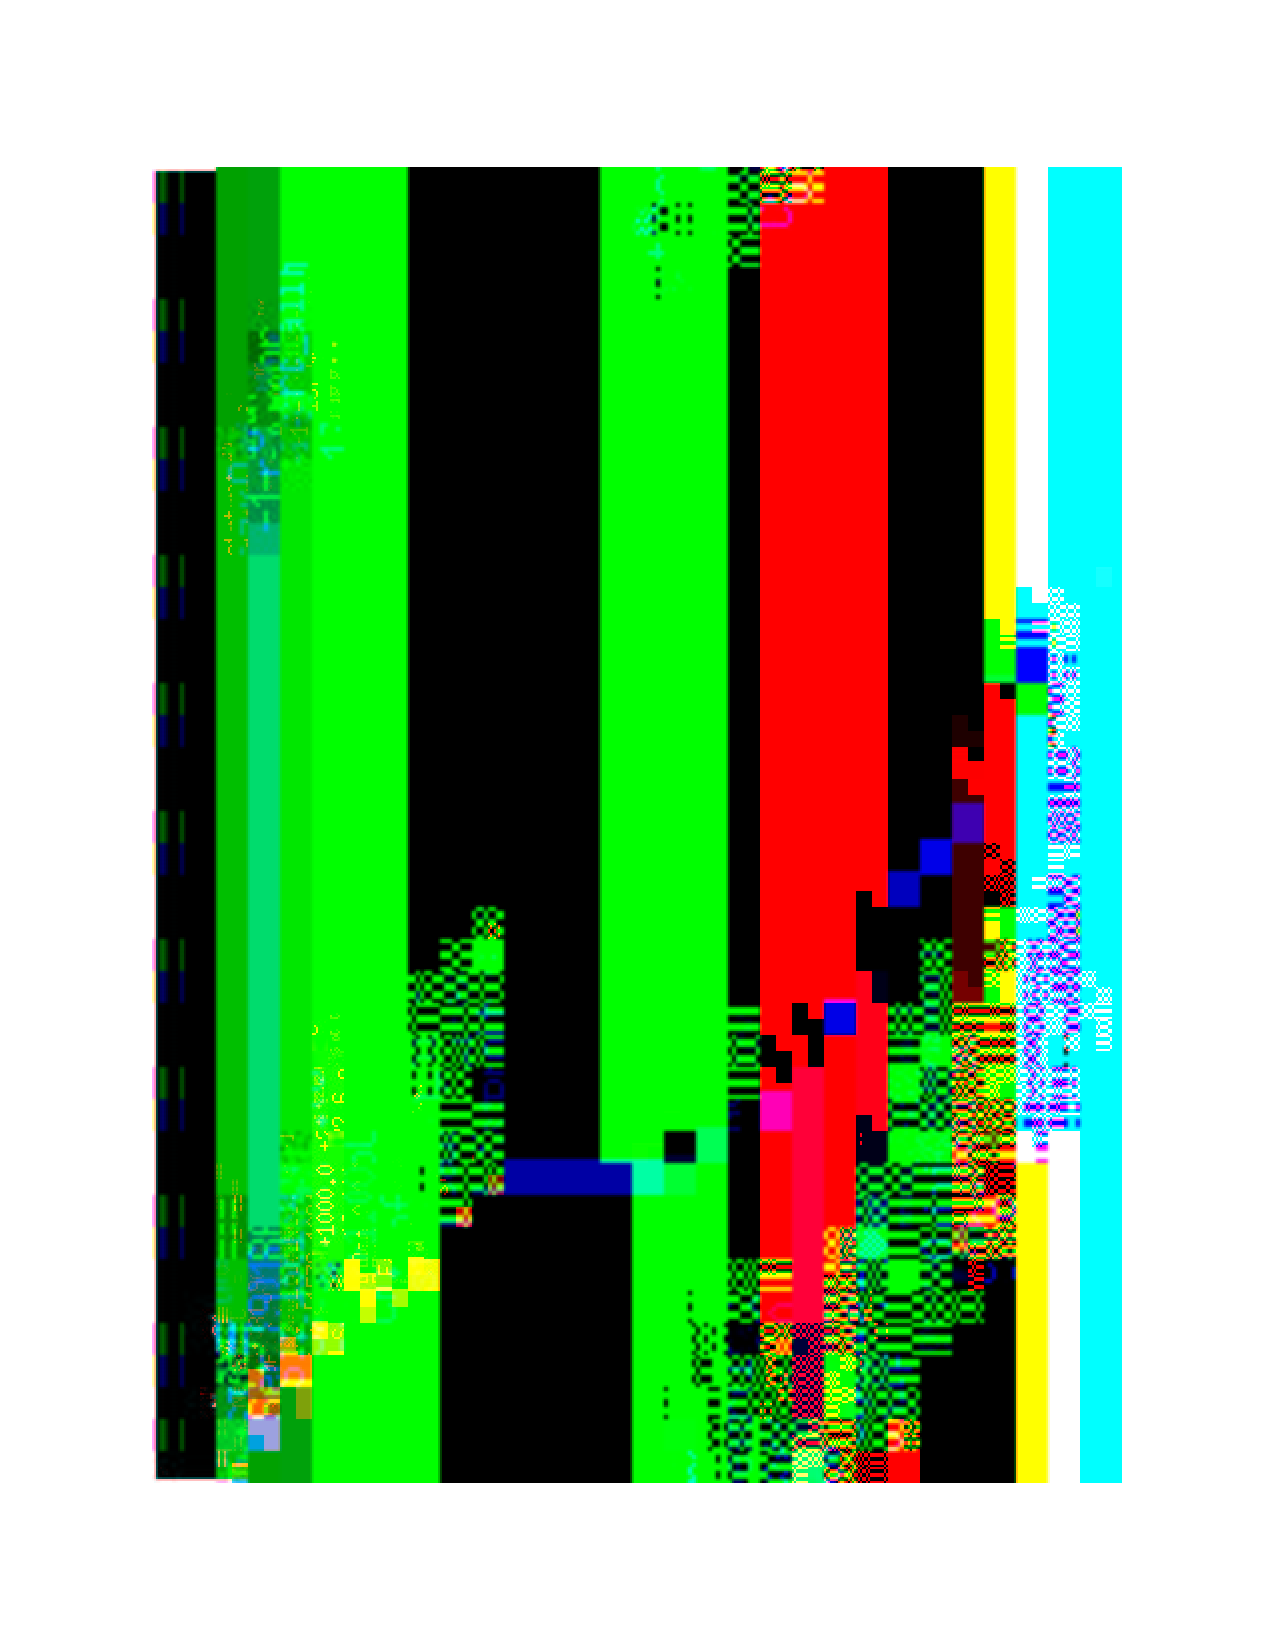
\includegraphics{nmonitor.pdf}}
\end{center}
\caption{\label{fig:nmonitor}Obrazovka nmonitoru}
\end{figure}

\chapter{Pou�it� prost�edky, p�evzat� k�d}

\section{V�vojov� prost�edky}

Pro psan� ve�ker�ho k�du byl pou��v�n editor ViM.

Makefile jsou generov�ny prost�ednictv�m bal�k� Autoconfig a
Automake. Konfigura�n� skript pro Autoconfig byl vytvo�en ze skriptu
generovan�ho programem autoscan, kter� je sou��st� Autoconfigu.

V�echny programy jsou verzov�ny v CVS. Verzov�n� doporu�uje kniha
\cite{telcontrol}. V�hody verzov�n� se uk�zaly p�i soub�n�m v�voji na v�ce
po��ta��ch. K�dov�n� prob�halo na t�ech po��ta��ch v Ond�ejov�, n�kolika
osobn�ch po��ta��ch v Praze a na po��ta��ch ve �pan�lsku.

Pro generov�n� WWW str�nek jsou pou�ity PHP skripty. Pro jejich
spr�vnou funkci je nutn� m�t nainstalovanou verzi PHP vy��� ne� 4.3.

Skripty b�� pod HTTP serverem Apache.

Data jsou ukl�d�na do (post-)rela�n� datab�ze PostgreSQL.

\section{Pou�it� knihovny}

Pro v�po�et astronomick�ch sou�adnic je pou�ita knihovna \cite{libnova}. V t�to
knihovn� bylo autorem opraveno n�kolik chyb a implementov�no n�kolik nov�ch
funkc�.  P�esn� p�ehled oprav je mo�n� z�skat z CVS repository libnovy,
dostupn�ho i p�es jej� WWW str�nky.

Pro z�pis a �ten� sn�mk� do form�tu fits je pou�ita knihovna cfitsio.
Pro pr�ci s WCS informacemi obsa�en�mi v hlavi�k�ch sn�mku je pou�ita knihovna
libwcs.

Pro zobrazov�n� informac� na termin�lu je pou�ita knihovna ncurses a knihovna
panel.

Pro p��stup na datab�zi jsou pou�ity knihovny, obsa�en� v distribuci
PostgreSQL.

\section{P�evzat� a pou�it� k�d, integrovan� p��mo do RTS2}

Z k�du syst�mu RTS1 byl p�evzat k�d pro ��zen� mont�e LX200. Pro RTS1 byl
tento k�d autorem p�epsan� ze zdrojov�ho k�du pluginu do programu XEphem,
napsan�m v jazyce C do jazyka Python. Pro pot�eby RTS2 byl autorem znovu m�rn�
upraven a p�eps�n zp�t do jazyka C.

Od magistra Martina Jel�nka poch�z� knihovna pro ovl�d�n� CCD kamer firmy SBIG,
knihovna pro ovl�d�n� mont�e Paramount, portovan� ze zdrojov�ch k�d� ur�en�ch
pro OS Windows do k�du p�elo�iteln�ho na Linuxu. Od Martina Jel�nka a koleg� ze
�pan�lska poch�z� t� bal�k pro astronometrii.

Od Scotta Barthelmy, Michaela Robbinse (oba pracuj� v Goddardov� st�edisku
��zen� vesm�rn�ch let� NASA) a Jamesa Kuypera (University of Michigan) poch�z�
k�d pro p��jem GRB pozic, kter� byl autorem t�to diplomov� pr�ce modifikov�n a
za�len�n do k�du grbc.

Od pracovn�k� ISDC\footnote{Integral Science Data Center} poch�z� k�d klienta
pro p��jem UDP paket� s informacemi o GRB detekovan�ch dru�ic� Integral, kter�
byl t� za�len�n do k�du grbc.

\section{Vlastn� k�d}

K�d knihovny pro s��ovou komunikaci, centr�ln�ho serveru, za��zen�, klient� pro
p��jem GRB, dlouhodob�ho pl�nova�e a monitorovac�ch klient�, SQL skripty pro
vytvo�en� datab�ze a pr�ci s datab�z� a k�d PHP str�nek umo��uj�c�ch p��stup do
datab�ze byl navr�en a naps�n v�lu�n� autorem t�to diplomov� pr�ce.

\chapter{Jin� syst�my, srovn�n�}

\section{Zm�ny oproti RTS1}

Zm�ny jsou sumarizov�ny v tabulce \ref{tab:rts12}.

\begin{table}[h!]
\begin{tabular}{p{7cm}|p{7cm}}
{\bf RTS1 {\it (ro�n�kov� projekt)}}		& {\bf RTS2 {\it (diplomov� pr�ce)}} \\
\hline
\hline
monolit					& modul�rn� \\ 
\hline
od n�vrhu v�z�no na konkr�tn� dalekohled, zm�ny mo�n�, ale n�ro�n�	& nen� v�z�no na konkr�tn� dalekohled, zm�ny mo�n� a relativn� snadn� \\
\hline
Python, bash				& C, bash, perl, PHP, SQL \\
\hline
kolem 5 tis�c ��dk� Pythonu		& kolem 13 tis�c vlastn�ch ��dk� zdrojov�ho k�du v jazyce C\footnote{v�etn� koment���}, celkem s p�evzat�m k�dem (ovlada�e kamer, p��jem GRB zpr�v) kolem 25 tis�c C ��dk� \\
\hline
pouze WWW rozhrann�			& WWW rozhran�, textov� monitoring \\
\hline
textov� datab�ze			& {\it (post)}rela�n� datab�ze - PostgreSQL \\
\hline
bez astrometrie sn�mk�			& s astrometri� sn�mk� \\
\hline
bez zp�tn� vazby p�es astrometrii	& se zp�tnou vazbou p�es astrometrii \\
\hline
bez automatick�ho po�izov�n� flat-fieldu		& s automatick�m po�izov�n� flat-fieldu \\
\hline
p�eru�iteln� po dokon�en� operace na kame�e (vy�ten� sn�mku, dokon�en� expozice) �i p�esunu dalekohledu	& p�eru�iteln� v jak�koliv okam�ik \\
\hline
nejasn� definovan� stavy, neobsahuje stavy pro flat-filedy, standbay, off 		& standby a off stavy \\
\hline
verzov�n dodate�n� v CVSku		& v CVSku verzov�n od po��tku \\
\hline
sou��st� projektu byly v praxi nikdy nepou�it� matlabovsk� algoritmy pro detekci hv�zd, planetek a optick�ch prot�j�k�	& syst�m vyu��v� pro tyto �koly dostupn� bal�ky pro zpracov�n� astronomick�ch sn�mk� \\
\hline
kolem tis�ce ��dk� Matlabovsk�ho k�du pro zpracov�n� sn�mk� & nespo��tan� mno�stv� zdrojov�ch ��dk� ciz�ch bal�k� pro astrometrii, prohl��en� sn�mk�, zpracov�n� sn�mk� \\
\end{tabular}
\caption{\label{tab:rts12}Srovn�n� RTS1 a RTS2}
\end{table}

Spr�vnost modul�rn� koncepce byla ov��ena ve �pan�lsku, kde bylo b�hem zhruba
dvou hodin integrov�no a odzkou�eno ovl�d�n� nov� mont�e Paramount, ke kter�
byly poskytnuty n�zko�rov�ov� ovlada�e.

Syst�m je pom�rn� jedine�n� integrac� kamery a dalekohledu tak, �e sn�mky jsou
automaticky opat�ov�ny sou�adnicemi. P�esto�e se tato �loha jev� jako
trivi�ln�, zna�n� procento sv�tov�ch dalekohled� nen� touto integrac� vybaveno.

\chapter{Sou�asn� stav}

Zad�n� pro ro�n�kov� projekt je mo�n� nal�zt v~p�iloze. 

Sou�asn� k�d je napsan� v~jazyce \cite{python-home}. K�d je pln� funk�n� a
spl�uje z�kladn� po�adavky, kter� na n�j byly v~zad�n� projektu kladeny:

\begin{itemize}
\item ovl�d� dalekohled a kameru
\item um� p�ij�mat zpr�vy o~nov�ch gama z�blesc�ch
\item v~rozumn� �as \footnote{maxim�ln� do p�ti minut, z�le�� na pr�behu
expozice} dok�e p�eru�it pr�v� prob�haj�c� pozorov�n� a v�novat se pozorov�ni
s~vy��� prioritou 
\item vytv��� archiv sn�mk�
\item um� po�izovat automaticky temn� sn�mky
\end{itemize}

Mimo to poskytuje n�kolik u�ite�n�ch funkc�, jeji� nutnost se prok�zala p�i
rutinn�m pozorov�n�. V�t�ina nebyla v~zad�n� ro�n�kov�ho projektu, a v�t�ina
byla doimplementov�na autorem diplomov� pr�ce po obh�jen� projektu.

\begin{itemize}
\item mo�nost automaticky zah�jit pozorov�n� p�i z�padu slunce
\item auto parking, 
\end{itemize}

Sou�asn� stav nejl�pe vystihuje n�sleduj�c� diagram:

\dia{rts-1-packages}{graf z�vislost� rts-1}


% \section{Ond�ejov - ovl�d�n� 2m dalekohledu}

\section{Ond�ejov - ovl�d�n� 60cm dalekohledu}

Ond�ejovsk� 60cm dalekohled slou�� pro pozorov�n� planetek a prom�nn�ch hv�zd.

Mont� dalekohledu je vybavena senzory. Dalekohled m� kupuli se �t�rbinou,
nat��en� kopule a pohyb dalekohledu ovl�d� po��ta� b��c� pod opera�n�m
syst�mem MS DOS. Pro ka�dou noc je p�ipraven seznam c�l�, z kter�ch je mo�n�
vyb�rat dal�� pozorov�n�.

Vy��t�n� kamery b�� pod opera�n�m syst�mem Windows, je ovl�d�no ru�n�. Sn�mky
jsou ukl�d�ny na pevn� disk, kter� je p��stupn� ze s�t�.

Zpracov�n� sn�mk� se d�je v poloautomatick�m re�imu. U dalekohledu je um�st�n
server slou��c� pro ukl�d�n� nam��en�ch sv�teln�ch k�ivek. 

Po��zen� sn�mky jsou archivov�ny na CD-ROM. Lze je dohledat z pozorovac�ch
protokol�.

Nev�hody:

\begin{description}

\item nen� vy�e�ena integrace dalekohledu a kamer

\item nen� mo�n� pln� automatick� pozorov�n�

\end{description}


% \section{Kle�}

\section{BOOTES - �pan�lsko}

Ve �pan�lsku, pod organizac� INTA\footnote{INTA - Institucion
National Technica in Astrofizica}, existuje podobn� projekt jako na
Ond�ejov�. Jedn� se tak� o~dalekohledy Meade, kamery SBIG. Ovl�d�n�
v~sou�asn� dob�, po p�tilet�m v�voji, b�� na heterogenn� s�ti s~OS
Windows a Linux.

Ovl�d�n� tvo�� n�kolik samostatn�ch proces�. Jsou pops�ny n��e:

\begin{itemize}

\item[TCM] Telescope Control Module - ��d� podle p�edem generovan�ho pl�nu pohyb
dalekohledu. Dalekohledem pohybuje pouze v~okam�iku, kdy nedoch�z� k~��dn�
expozici. P�i p��chodu zpr�vy o~z�blesku okam�it� p�esouv� dalekohled na novou
pozici, bez ohledu na pr�v� prob�haj�c� expozice. Naps�n v~jazyce C, b�� na
Linuxu.

\item[DCM] Dome Control Module - ovl�d� st�echu, kontroluje stav po�as� pomoc�
meterologick� v�e, hl�s� stav st�echy a po�as� p�es SMS br�nu, hl�s� otv�r�n�
a zav�r�n� st�echy TCM. Naps�n pod LabView, b�� na Windows 98. 

\item[OTM] Optical Transient Monitor - ��d� sn�mkov�n�. Sou��st� programu jsou
funkce pro automatick� po�izov�n� a zpracov�n� kalibra�n�ch sn�mk�. V~sou�asn�
dob� se pou��v� pouze na po�izov�n� sn�mk� (jak kalibra�n�ch, tak oby�ejn�ch),
jejich dal�� zpracov�n� pou�it� ��d� linuxovsk� pipeline. Ps�n v~Borland C++
Builderu s~pou�it�m knihovny OWL, b�� na Windows 98. 

\item[IAM] Image Analysis Monitor - pipeline postaven� na programech z~Opery,
umo��uj�c� zpracov�n� sn�mk�, jejich astrometrii a fotometrii. V~sou�asn� dob�
se pou��v� pouze na astrometrii.  Ps�n kombinac� linuxov�ch prost�edk� (z�klad
v~jazyce C, ��zen� p�es Bashovsk� a Perl skripty).

\dia{bootes}{Sch�ma komunikace syst�mu BOOTES}

\end{itemize}

Nev�hody:

\begin{itemize}
\item neexistence jednot�c�ho protokolu
\item dalekohled nem��e kontorolovat kamery, pr�m�rn� doba mezi ukon�en�m
p�esunu dalekohledu a po��zen�m prvn�ho sn�mku bude o~trochu v�t�� ne� jedna
polovina celkov� doby na expozizi a vy�ten� sn�mku \footnote{Po p�esunu na
novou pozici m��e b�t kamera v~jak�mkoliv stavu. V~nejlep��m p��pad� pr�v�
doko�ila vy�ten� CCD �ipu a pr�v� se chyst� zah�jit novou expozici,
v~nejhor��m zah�jila p�ed chv�l� expozici, bude vy��tat, pot� po��d� temn�
sn�mek a teprve pot� bude exponovat. V~pouze o~trochu m�n� hor��m p��pad� p�ed
chv�l� zah�jila expozici, bude vy��tat a teprve po t� exponovat. ????P�esn�
v�po�et?????????}
\item nestabilita Windowsovsk�ho vy��ta�e SBIGovsk�ch kamer, dan� vlastnostmi
GUI a pom�rn� slo�it�m k�dem.
\item nemo�nost vy��tat dv� kamery na jednom po��ta�i sou�asn�, empiricky
ov��en� - OS Windows nezvl�d� po��dn� p�id�lov�n� �asu na CPU a podobn� pokusy
vedou k~p�du syst�mu. V~sou�asn� konfiguraci �e�ena sou�asnou expoc� dvou
kamer, a jejich n�sledn�m postupn�m vy��t�n�m, druh� sn�mek je pak ale hrozn�
za�um�n�.
\item ne�e�� probl�my s~ost�en�m kamer
\end{itemize}


\section{Nightview - Monte Boo, Brno}

Program umo��uje ovl�d�n� SBIGovsk�ch kamer. Pou��v� vlastn� protokol pro
jejich ovl�d�n� p�es Internet, je rozd�len na klientskou a serverovou ��st.
Nekombinuje ovl�d�n� dalekohledu, na to je program Telescope control.

Umo��uje v~pohodln�m GUI ��dit expozici kamer, um� z�kladn� zobrazov�n�
sn�mku.

Nev�hody

\begin{itemize}
\item s~kamerou nen� mo�n� komunikovat p�i pos�l�n� dat.
\item nen� �e�ena integrace dalekohledu s kamerou
\item nen� �e�ena automatizace pozorov�n�
\end{itemize}


% \section{ROTSE}

%\section {LINEAR - Lincoln Near Earth Asteroid Registry}

Dalekohled, um�st�n� na Lincoln Observatory v~USA. Jeho hlavn�m c�lem
je hled�n� nov�ch asteroid�. zvl�t� pak t�ch, kter� by mohli
potenci�ln� ohrozit zemi - bl�zkozemn�ch asteroid� \footnote{NEA -
Near Earth Asteroids}.


% \section{Nova}

% \section{HUT}

\appendix

\chapter{P��kazy}

\def\comname#1#2#3{
{\bf #1} {\it #2} #3
\newline}

\def\comvalue#1#2#3{
{\it #1} { #2} #3
\newline}

\def\comret#1#2{
{\it E:}{\bf #1} #2
\newline}

\section{Konvence}

{\bf Tu�ne} je vys�zeno jm�no p��kazu a jm�no n�vratov� hodnoty.

{\it Kurz�vou a v [hranat�ch z�vork�ch]} jsou vys�zeny parametry
p��kazu, a n�vratov� hodnoty na ��dce.

\section{Obecn� n�vratov� hodnoty}

Za��zen� vrac� 0, pokud po�adovan� operace prob�hla �sp�n�. Pokud
p��kaz neexistuje, nebo klient nen� autorizov�n pro prov�d�n� dan�ho
p��kazu, vrac� hodnotu DEVDEM\_E\_COMMAND. Pokud je pro p��kaz zad�n
nespr�vn� po�et parametr�, vrac� hodnotu DEVDEM\_E\_PARAMSVAL.

\section{Serverd}

\subsection{Inicializa�n� p��kazy}

\comname{login}{[jm�no u�ivatele]}{p�ihl�s� u�ivatele do syst�mu}
\comret{DEVDEM\_E\_COMMAND}{klient je ji� p�ihl�en nebo registrov�n}
\comret{DEVDEM\_E\_SYSTEM}{nen� mo�n� p�ihl�sit dal��ho u�ivatele}

\comname{password}{[heslo]}{po�le heslo u�ivatele}
\comvalue{logged\_as}{[��slo spojen�]}{��slo spojen� na stran� serveru,
pou��van� pro dal�� autentifikaci}
\comvalue{I status\_num}{[po�et stav�]}{}
\comvalue{I status}{[��slo stavu] [n�zev stavu] [sou�asn� hodnota stavu]}{}
\comret{DEVDEM\_E\_SYSTEM}{heslo neodpov�d�}

\comname{register}{[jm�no za��zen�] [typ za��zen�] [host]:[port]}{zaregistruje nov� za��zen�}
\comret{DEVDEM\_E\_SYSTEM}{za��zen� se stejn�m jm�nem je ji�
zargistrov�no}

\subsection{Informa�n� p��kazy}

\comname{info}{}{vyp��e informace o p�ipojen�ch za��zen�ch a p�ipojen�ch klientech}
\comvalue{user}{[id] [priorita] [*|-] [jm�no u�ivatele] [popis prov�d�nn� �innosti]}
{informace o p�ipojen�m u�ivateli - jeho ��slo, priority, zda je klientem s
nejvy�� prioritou �i ne, a stru�n� popis, o jak�ho klienta se jedn�}
\comvalue{device}{[��slo za��zen�] [jm�no za��zen�] [host]:[port] [typ za��zen�]}
{informace o p�ipojen�m za��zen�}
 
\comname{key}{[jm�no za��zen�]}{vy��d� si kl�� pro autorizaci}
\comvalue{authorization\_key}{[jm�no za��zen�] [kl��]}{autoriza�n�
kl�� pro dan� za��zen�}
\comret{DEVDEM\_E\_SYSTEM}{za��zen� neexisuje}

\comname{priority}{[nov� priorita]}{zm�n� prioritu dan�ho spojen�}
\comvalue{old\_priority}{[hodnota priority]}{sou�asn� priorita spojen�}
\comvalue{actual\_priority}{[��slo spojen� dr��c�ho prioritu]
[hodnota jeho priority]}{spojen� s nejv�t�� prioritou}
{new\_priority}{[��slo spojen� dr��c� prioritu] [hodnota priority]}
{spojen� s prioritou po proveden� zm�ny}
\comret{DEVDEM\_E\_PRIORITY}{pokud zm�na priority nemohla prob�hnout}

\comname{prioritydeferred}{[nov� priorita]}{provede zm�nu odlo�enou
zm�nu priroty}

\comname{on}{}{zm�n� stav serveru na jeden z opera�n�ch stav�, v
z�vislosti na aktu�ln�m �ase a datu}

\comname{off}{}{zm�n� stav serveru na off - vypnuto}

\section{Za��zen� - obecn� komunikace}

Pokud nen� klient autorizov�n, vrac� v�echna komunikace hodnotu
DEVDEM\_E\_SYSTEM.

Pokud dojde p�i vykon�v�n� p��kazu k chyb� v komunikaci se za��zen�m,
vrac� se hodnota DEVDEM\_E\_HW.

\comname{auth}{[��slo spojen�] [autentifika�n� kl��]}{provede
autorizaci}
\comvalue{I status\_num}{[po�et stav�]}{}
\comvalue{I status}{[��slo stavu] [jm�no stavu] [hodnota stavu]}{}
{informace o stavu za��zen�}{}
\comret{DEVDEM\_E\_SYSTEM}{pokud autorizace neprob�hla}

\comname{ready}{}{zjist�, jestli je za��zen� p�ipojeno. Je mo�n� volat
opakovan�.}

\comname{help}{}{vyp��e n�pov�du}

\comname{exit}{}{ukon�� spojen�}

\comname{blockstart}{}{informuje za��zen� o za��tku bloku, nutn� pro
proveden� odlo�en� zm�ny priority}
\comret{DEVDEM\_E\_SYSTEM}{pokud je spojen� ji� v bloku}

\comname{blockcheck}{}{odlo�en� zm�na priority je mo�n�}
\comret{DEVDEM\_E\_SYSTEM}{pokud nen� spojen� v bloku}

\comname{blockend}{}{ukon�en� bloku pro odlo�enou zm�nu priority}
\comret{DEVDEM\_E\_SYSTEM}{pokud spojen� nen� v bloku}

\section{Kamera}

\comname{info}{}{vyp��e informace o kame�e}
\comvalue{type}{[typ kamery]}{}
\comvalue{serial}{[s�riov� ��slo kamery]}{}
\comvalue{chips}{[po�et �ip� kamery]}{}
\comvalue{temperature\_regulation}{[CAMERA\_COOL\_HOLD|CAMERA\_COOL\_MAX|CAMERA\_COOL\_OFF]}{stav
chazen� kamery}
\comvalue{temperature\_setpoint}{[teplota]}{teplota, na kterou se
kamera sna�� chladit}
\comvalue{air\_temperature}{[teplota]}{hodnota teplotn�ho �idla,
ud�vaj�c�ho teplotu vzducju}
\comvalue{ccd\_temperature}{[teplota]}{teplota CCD �ipu}
\comvalue{cooling\_power}{[promile v�konu]}{hodnota hlazen�}
\comvalue{fan}{[0|1]}{stav v�tr�ku kamery}

\comname{chipinfo}{[��slo �ipu]}{vrac� informace o dan�m �ipu}
\comvalue{chip [��slo �ipu] width}{[���ka]}{���ka �ipu}
\comvalue{chip [��slo �ipu] height}{[v��ka]}{v��ka �ipu}
\comvalue{chip [��slo �ipu] binning\_vertical}{[vertik�ln� binning]}{}
\comvalue{chip [��slo �ipu] binning\_horizontal}{[horizont�ln�
binning]}{}
\comvalue{chip [��slo �ipu] pixelX}{[rozm�r pixelu v X sm�ru]}{}
\comvalue{chip [��slo �ipu] pixelY}{[rozm�r pixelu v Y sm�ru]}{}
\comvalue{chip [��slo �ipu] gain}{[zisk v e/ADU]}{}

\comname{expose}{[��slo �ipu] [sv�tl�/tmav� sn�mek] [expozi�n�
�as]}{zah�j� na dan�m �ipu expozici}

\comname{stopexpo}{[��slo �ipu]}{ukon�� expozici}

% \comname{progexpo}{[��slo �ipu]}{vrac� informace o prob�haj�c�
% expozici}

\comname{binning}{[��slo �ipu] [vertik�ln� binning] [horizont�ln�
binning]}{zm�n� binning �ipu}

\comname{readout}{[��slo �ipu]}{zah�j� vy��tan� �ipu}
\comvalue{D connect}{[��slo spojen�] [host]:[port] [velikost dat]}
{informace o nutnosti nav�zat datov� spojen� na dan� port}
P��kaz skon�� a� po �sp�n�m nav�z�n� spojen�.

\comname{stopread}{[��slo �ipu]}{ukon�� vy��t�n� dan�ho �ipu}

\comname{cooltemp}{[temperature]}{nastav� teplotu chlazen� �ipu}

\section{Mont�}

\comname{set}{[RA] [DEC]}{nastav� pozici mont�e}

\comname{move}{[RA] [DEC]}{zah�j� p�esun mont�e na novou pozici}

\comname{info}{}{vyp��e informace o mont�i}
\comvalue{type}{[typ dalekohledu]}{}
\comvalue{serial\_number}{[s�riov� ��slo mont�e]}
\comvalue{ra}{[RA]}{hodnota rektascenze mont�e}
\comvalue{dec}{[DEC]}{hodnota deklinace mont�e}
\comvalue{park\_dec}{[DEC]}{parkovac� deklinace}
\comvalue{longtitude}{[zem�pisn� d�lka]}{zem�pisn� d�lka dalkohledu}
\comvalue{latitude}{[zem�pisn� ���ka]}{zem�pisn� ���ka dalekohledu}
\comvalue{siderealtime}{[�as]}{m�stn� hv�zdn� �as v okam�iku
pozorov�n�}
\comvalue{localtime}{[�as]}{ob�ansk� �as v m�st� pozorov�n�}
\comvalue{correction\_mark}{[��slo korekce]}{��slo posledn� prob�hnut�
korekce}

\comname{park}{}{zaparkuje dalekohled}

\section{P��klad komunikace}

M�me jedno za��zen�, kter� se jmenuje C0 a je CCD kamerou. K tomuto za��zen�
se p�ipojuje jeden klient, kter� je chce prov�d�t ost�en� kamery. Po sv�m
p�ipojen� se pokus� z�skat prioritu, zm�n� teplotu chlazen� kamery a provede
expozici n�sleduj�c� vy�ten�m z�skan�ho sn�mku.

Jm�no u�ivatele je petr, jeho heslo je 123456.

Kamera je um�st�na na po��ta�i se jm�nem c0, jej� server b�� na portu 5556.
Datov� porty za��naj� portem 5557.

V n�sleduj�c�m p��klad� zna�� {\bf k} klienta, {\bf S} centr�ln� server a {\bf
C0} kameru. Komunikace a je jej� sm�r je ur�en pomoc� =>. 

\def\conn#1#2#3{
{\bf #1} => {\bf #2} - #3
\newline
}

Nap��klad:

\conn{k}{S}{command 1}

znamen� text "command 1" poslan� klientem centr�ln�mu serveru.

\conn{C0}{S}{register C0 3 c0:5556}
\conn{S}{C0}{I status\_num 1}
\conn{S}{C0}{I status 0 server\_st 2}
Centr�ln� server zd�lil kame�e, �e m� jeden stav, jeho jm�no je server\_st a
jeho hodnota je rovn� 1.
\conn{S}{C0}{+000 Success}

\conn{k}{S}{login petr}
\conn{S}{k}{+000 Success}
\conn{k}{S}{password 123456}
\conn{S}{k}{logged\_as 0}
\conn{S}{k}{I status\_num 1}
\conn{S}{k}{I status 0 server\_st 2}
\conn{S}{k}{+000 Success}

\conn{k}{S}{info}
\conn{S}{k}{user 0 petr -1 -}
\conn{S}{k}{device 0 C0 c0:5556 3}
\conn{S}{k}{+000 Success}
Je p�ipojen jeden u�ivatel - to je na�e spojen�, a jedno za��zen� - c0.

\conn{k}{S}{key C0}
\conn{S}{k}{authorization\_key 23456}
\conn{S}{k}{+000 Success}

Klient po��dal o autoriza�n� kl��.

\conn{k}{C0}{auth 0 23456}
\conn{C0}{S}{authtorize 0 23456}
\conn{S}{C0}{authorization\_ok 0}
\conn{S}{C0}{+000 Success}

Server potvrdil pravost kl��e pro klienta.

\conn{C0}{k}{I status\_num 3}
\conn{C0}{k}{I status 0 img\_chip 0}
\conn{C0}{k}{I status 1 trc\_chip 0}
\conn{C0}{k}{I status 2 priority 0}
\conn{C0}{k}{+000 Success}

Klient byl autorizov�n, kamera mu zd�lila po�et, n�zvy a hodnoty stav�.

\conn{k}{C0}{ready}
\conn{C0}{k}{+000 Success}

\conn{k}{C0}{info}
\conn{C0}{k}{type ST8}
\conn{C0}{k}{serial  819901486}
\conn{C0}{k}{chips 2}
\conn{C0}{k}{temperature\_regulation 0}
\conn{C0}{k}{temperature\_setpoint 1000.0}
\conn{C0}{k}{air\_temperature 17.39}
\conn{C0}{k}{ccd\_temperature 13.51}
\conn{C0}{k}{cooling\_power 0}
\conn{C0}{k}{fan 0}
\conn{C0}{k}{+000 Success}

\conn{k}{C0}{cooltemp -10}
\conn{C0}{k}{+000 Success}

\conn{k}{C0}{expose 0 1 120}
\conn{C0}{k}{S img\_chip 1 exposure chip started}
\conn{C0}{k}{+000 Success}

\conn{C0}{k}{S img\_chip 4 exposure chip finished}

\conn{k}{C0}{readout 0}
\conn{C0}{k}{D connect 8 C0:5565 3145784}

Klient vytvo�� datov� spojen� a za�ne na n�m p�ij�mat data. Data budou dlouh�
3145784 byt�.

\conn{C0}{k}{S img\_chip 2 reading chip started}
\conn{C0}{k}{+000 Success}

\conn{C0}{k}{S img\_chip 0 reading chip finished}

Server odeslal posledn� data, klient mus� p�e��st v�echny data z datov�ho
spojen� a porovnat je s d�lkou dat, kterou obdr�el na za��tku spojen�.


\chapter{Pou�it� prost�edky, p�evzat� k�d}

\section{V�vojov� prost�edky}

Pro psan� ve�ker�ho k�du byl pou��v�n editor ViM.

Makefile jsou generov�ny prost�ednictv�m bal�k� Autoconfig a
Automake. Konfigura�n� skript pro Autoconfig byl vytvo�en ze skriptu
generovan�ho programem autoscan, kter� je sou��st� Autoconfigu.

V�echny programy jsou verzov�ny v CVS. Verzov�n� doporu�uje kniha
\cite{telcontrol}. V�hody verzov�n� se uk�zaly p�i soub�n�m v�voji na v�ce
po��ta��ch. K�dov�n� prob�halo na t�ech po��ta��ch v Ond�ejov�, n�kolika
osobn�ch po��ta��ch v Praze a na po��ta��ch ve �pan�lsku.

Pro generov�n� WWW str�nek jsou pou�ity PHP skripty. Pro jejich
spr�vnou funkci je nutn� m�t nainstalovanou verzi PHP vy��� ne� 4.3.

Skripty b�� pod HTTP serverem Apache.

Data jsou ukl�d�na do (post-)rela�n� datab�ze PostgreSQL.

\section{Pou�it� knihovny}

Pro v�po�et astronomick�ch sou�adnic je pou�ita knihovna \cite{libnova}. V t�to
knihovn� bylo autorem opraveno n�kolik chyb a implementov�no n�kolik nov�ch
funkc�.  P�esn� p�ehled oprav je mo�n� z�skat z CVS repository libnovy,
dostupn�ho i p�es jej� WWW str�nky.

Pro z�pis a �ten� sn�mk� do form�tu fits je pou�ita knihovna cfitsio.
Pro pr�ci s WCS informacemi obsa�en�mi v hlavi�k�ch sn�mku je pou�ita knihovna
libwcs.

Pro zobrazov�n� informac� na termin�lu je pou�ita knihovna ncurses a knihovna
panel.

Pro p��stup na datab�zi jsou pou�ity knihovny, obsa�en� v distribuci
PostgreSQL.

\section{P�evzat� a pou�it� k�d, integrovan� p��mo do RTS2}

Z k�du syst�mu RTS1 byl p�evzat k�d pro ��zen� mont�e LX200. Pro RTS1 byl
tento k�d autorem p�epsan� ze zdrojov�ho k�du pluginu do programu XEphem,
napsan�m v jazyce C do jazyka Python. Pro pot�eby RTS2 byl autorem znovu m�rn�
upraven a p�eps�n zp�t do jazyka C.

Od magistra Martina Jel�nka poch�z� knihovna pro ovl�d�n� CCD kamer firmy SBIG,
knihovna pro ovl�d�n� mont�e Paramount, portovan� ze zdrojov�ch k�d� ur�en�ch
pro OS Windows do k�du p�elo�iteln�ho na Linuxu. Od Martina Jel�nka a koleg� ze
�pan�lska poch�z� t� bal�k pro astronometrii.

Od Scotta Barthelmy, Michaela Robbinse (oba pracuj� v Goddardov� st�edisku
��zen� vesm�rn�ch let� NASA) a Jamesa Kuypera (University of Michigan) poch�z�
k�d pro p��jem GRB pozic, kter� byl autorem t�to diplomov� pr�ce modifikov�n a
za�len�n do k�du grbc.

Od pracovn�k� ISDC\footnote{Integral Science Data Center} poch�z� k�d klienta
pro p��jem UDP paket� s informacemi o GRB detekovan�ch dru�ic� Integral, kter�
byl t� za�len�n do k�du grbc.

\section{Vlastn� k�d}

K�d knihovny pro s��ovou komunikaci, centr�ln�ho serveru, za��zen�, klient� pro
p��jem GRB, dlouhodob�ho pl�nova�e a monitorovac�ch klient�, SQL skripty pro
vytvo�en� datab�ze a pr�ci s datab�z� a k�d PHP str�nek umo��uj�c�ch p��stup do
datab�ze byl navr�en a naps�n v�lu�n� autorem t�to diplomov� pr�ce.

\chapter{Zad�n� projektu}

N�zev:
 Detekce astronomick�ch objekt� s~prom�nnou intenzitou za pomoci robotick�ho teleskopu

\begin{enumerate}

\item ��astn�c� projektu

\begin{itemize}
\item Vedouc�:	Mgr. Radim Hal��, halir@ms.mff.cuni.cz

\item Konzultanti:
		\newcommand\theitemi{}
		\begin{itemize}
			\item	RNDr. Ren� Hudec, ASU AV �R Ond�ejov, rhudec@asu.cas.cz
			\item Dr. Ing. Jan Sold�n, ASU AV �R Ond�ejov, jsoldan@asu.cas.cz
			\item Bc. Lenka �arounov�, ASU AV �R Ond�ejov, lenkas@asu.cas.cz
		\end{itemize}	

\item �e�itel�:
	\begin{itemize}
		\item Tom� J�lek, tjil6236@ss1000.ms.mff.cuni.cz
		\item	Petr Kub�nek, pkub6315@ss1000.ms.mff.cuni.cz
		\item Filip Krolupper, fkro6306@ss1000.ms.mff.cuni.cz
		\item Franti�ek Kvapil, fkva7312@ss1000.ms.mff.cuni.cz
	\end{itemize}	

\item T�mov� adresa: rtt@ss1000.ms.mff.cuni.cz
\end{itemize}


\item Vyps�n� projektu:
zimn� + letn� semestr 1999/2000


\item Zad�n�:
Navrhn�te a naimplementujte software pro vyhled�v�n� optick�ch prot�j�k� gama
z�blesk�. Na vstupu je zpr�va z~mezin�rodn�ho centra sleduj�c� pomoc� dru�ic
um�st�n�ch na ob�n� dr�ze gama z�blesky. Na v�stupu z~programu je odpov��,
zda se v~c�lov� oblasti vyskytuje �i nevyskytuje objekt podez�el� z~toho, �e
by mohl b�t poz�statkem gama z�blesku a jeho p��padn� sou�adnice a magnituda.
K~probl�mu pat�� t� evidence napozorovan�ch dat, p��stup k~nim a dal��
"rozumn�" �koly.


\item Z�kladn� ��sti projektu
\begin{itemize}
\item komunikace s~robotick�m teleskopem (nastaven�, sejmut� sn�mku, zji�t�n�
   stavu, atd.)
\item pl�nova� pozorov�n� v�etn� zpracov�n� mail� z~dru�ic detekuj�c�ch gama
  z�blesky
\item evidence proveden�ch pozorov�n� 
\item zpracov�n� sn�mk� v�etn� automatick� detekce zaj�mav�ch objekt�
  (p�edzpracov�n� sn�mk� pomoc� pr�m�rov�n� a flatfield/darkfield korekc�,
  radiometrick� a geometrick� kalibrace, hled�n� objekt� s~prom�nnou
  intenzitou)
\item (voliteln�) anal�za z�skan�ch dat: z�sk�n� sou�adnic objekt�, astrometrie,
  fotometrie, ...
\end{itemize}

\item Po�adavky na realizaci
\begin{itemize}
	\item platforma UNIX se snahou o~platformn� nez�vislost snaha vyu��t dostupn� SW prost�edky:
  \item SW pro ovl�d�n� teleskopu (od Jan Sold�na, komunikace pomoc� emailu)
  \item skriptovac� jazyky Python resp. Perl (nap�. pro pl�nova�)
  \item numerick� syst�my Matlab/Ocstave/Scilab (zpracov�n� sn�mk�)
  \item "low-level" programov�n� v~C
  \item dokumentace v~syst�mu TeX, pravd�podobn� anglicky
	\item sou��st� projektu bude i �e�en� relevantn�ch teoretick�ch probl�m�.
	\item P��padn� v�sledky by m�ly b�t publikov�ny ve form� odborn�ch �l�nk�.
\end{itemize}	


\item Pozn�mky k~realizaci (od Petra Kub�nka)

P�i psan� programu se budeme maxim�ln� sna�it pou��vat ji� existuj�c� software.
Podobn� operace jako budeme pot�ebovat my se d�laj� p�i pozorov�n� planetek �i
prom�nn�ch dvojhv�zd. 

Pozorovac� p�istroj budeme ovl�dat pomoc� n�jak�ho pom�rn� jednoduch�ho
rozhran�, na vstupu zad�me sou�adnice a za��zen�, kter�m budeme sn�mkovat,
jako v�stup obdr��me po��zen� sn�mek �i informace o~tom, �e sn�mek nebyl
po��zen a d�vod pro� k~tomu do�lo. Ovlada� na p��stroje d� k~dispozici
Ond�ejovsk� observato�.

Pl�nova� si nap��eme vlastn�. M�l by um�t n�sleduj�c�:
\begin{itemize}
   \item vstup ru�n�, automatick� (zpr�va ze st�ediska vyhodnocuj�c� informace
     z~dru�ic) a generovan� (dalekohled by se m�l s�m �kolovat)
   \item v�pis napl�novan�ch akc�
\end{itemize}	 

Z~evidence by m�lo b�t jasn�, kdy se co napozorovalo a s~jak�m v�sledkem.
Tak� by se m�lo evidovat, odkud se braly informace o~pozorovan�ch objektech
a jak� po�adavky na pozorov�n� do syst�mu vstoupily.

P�edzpracov�n� po��zen�ho sn�mku zahrnuje dv� z�kladn� operace - darkfield a
flatfield korekci. Jimi se odstra�uj� vady CCD �ipu. D�le p�ipad� v~�vahu
zaost�ov�n�, odstran�n� vlivu atmosf�ry a podobn�.

Podez�el� objekty se daj� vyhled�vat bu�to podle zm�ny jasnosti (magnituty)
na dvou sn�mc�ch po��zen�ch n�kolik minut po sob�, nebo srovn�v�n�m se
star��mi sn�mky p��padn� s~katalogy a hled�n�m nov�ch objekt�.

Datab�ze po��zen�ch sn�mk� by m�la umo��ovat vyhled�v�n� a zobrazovan�
po��zen�ch sn�mk� podle r�zn�ho krit�ria, operace se sn�mkem a podobn�.


\item Dodatek: gama z�blesky a jejich optick� prot�j�ky

Gama z��en� je nejenergi�t�j�� elektromagnetick� z��en�. Gama z�blesky jsou
prudk� a kr�tk� v�trysky tohoto z��en�, p�ich�zej�c� k~n�m z~vesm�ru. Z�blesky
trvaj� okolo jedn� sekundy. Jeliko� od gama z��en� je Zem� odst�n�na, mus�me
gama z�blesky hledat pomoc� p��stroj� na dru�ic�ch. V~p��pad� �sp�n� detekce
zn�me pouze p�ibli�nou polohu zdroje z�blesku, rozm�ry podez�el� oblasti se
pohybuj� ve stupn�ch (pro srovn�n� - m�s�c v~�pl�ku = p�l stupn�).

Optick�m prot�j�kem gama z�blesku se rozum� podez�el� objekt ve sm�ru gama
z�blesku pozorovan� ve viditeln�m spektru. Optick� prot�j�ek je pozorov�n u
zhruba poloviny p�esn� lokalizovan�ch zdroj� gama z�blesk�. M�l by b�t
pozorovateln� d�le ne� gama z�blesk - ur�it� minuty, mo�n� dny. Za jeden den
je detekov�n pr�m�rn� jeden gama z�blesk, z~r�zn�ch d�vod� (po�as�, um�st�n�
na neviditeln� ��sti oblohy, mal� jasnost, ..) u~v�t�iny nen� mo�no dohledat
optick� prot�j�ek - zat�m se jich poda�ilo dohledat pouze n�kolik.

Nen� jasn�, z~�eho gama z�blesk poch�z� - existuje zhruba 200 teoretick�ch
model�. N�kter� z~nich vych�z� z~n�jak� katastrofick� sr�ky n�sledovan�
v�buchem. P�i sr�ce vznik� gama z��en�, p�i v�buchu z~n�raz� rozp�naj�c�ch se
��stic poch�z� optick� z��en�. Optick� prot�j�ek by m�l tedy b�t pozorovateln�
o~trochu pozd�ji ne� gama z�blesk. Z~extrapolace nam��en�ch optick�ch
prot�j�k� gama z�blesk� vypl�v�, �e by mohl m�t po kr�tkou dobu dostate�nou
jasnost na to, aby byl viditeln� i triedrem �i mal�m astronomick�m p��strojem.

\end{enumerate}


\section{�asov� pl�n}

\begin{description}

\item[listopad 2001] za��tek hled�n� t�matu diplomov� pr�ce

\item[b�ezen 2002] schv�len� t�matu diplomov� pr�ce

\item[duben 2002] za��tek v�voje komunika�n� knihovny, za��tek verzov�n� v
CVSku

\item[srpen 2002] centr�ln� server

\item[listopad 2002] implementace a testy server� pro kamery a dalekohled,
datab�ze sn�mk�

\item[konec prosince 2002] prvn� pozorov�n�

\item[leden 2003] nmonitor, grbc

\item[�nor 2003] odstaven� RTS1 z BARTa

\item[duben 2003] dokon�ovac� pr�ce, oprava chyb, dopisov�n� a kompletace
dokumentace

\end{description}


\begin{thebibliography}{xxxxxx--9999}

	\bibitem[Python--2002]{python-home}
		Python home page - \href{http://www.python.org}
	\bibitem{martinez}
		Martinez/Klotz - A~practical Guide to CCD Astronomy
	\bibitem[Trueblood, Genet--1997]{telcontrol}
		Mark Trueblood, Russell Merle Genet - Telescope Control, Willmann-Bell 1997
	\bibitem{ratledge}
		David Ratledge - The Art and Science of CCD Astronomy
	\bibitem{RFC854}
		Telnet RFC - \href{http://www.rfc.net/rfc854.html}
	\bibitem{RFC959}
		FTP RFC - \href{http://www.rfc.net/rfc959.html}
\end{thebibliography}


\include{slovnik}

\listoffigures

% \include{doxygen/latex/refman}
% \newpage
% \printindex
\end{document}
